%!TEX TS-program = xelatex
%!TEX encoding = UTF-8 Unicode

% MICHAEL ELLIOT KING -x  PORTFOLIO

% HEADER
	\documentclass[12pt, landscape]{article}
	\usepackage{geometry} 
	\geometry{letterpaper, textwidth=8.5in, textheight=6in}

	\usepackage{fontspec} %OpenType fonts
	\usepackage[bookmarks, colorlinks, breaklinks, 
	pdftitle={Mechanical Engineering Portfolio - Michael Elliot King}, %title of the document
	pdfauthor={Michael Elliot King}] %author of the document
	{hyperref}
	\usepackage[usenames, dvipsnames]{xcolor} % colors
	\hypersetup{linkcolor=CadetBlue,citecolor=black,filecolor=black,urlcolor=CadetBlue} % Link colors
	\usepackage{xunicode} % Allows generation of unicode characters from accented glyphs
	\defaultfontfeatures{Mapping=tex-text} % Converts LaTeX specials (``quotes'' --- dashes etc.) to unicode
	\setromanfont {Helvetica Neue Light} % Main text font 

	\usepackage{setspace} %line spacing
	\linespread{1.4} %double space
	\setcounter{secnumdepth}{0} % sections are level 1 - i.e. no numbering but still in ToC

	\usepackage{pdflscape} %landscape
	\usepackage{pgfgantt} %gantt chart
	\usepackage[nottoc]{tocbibind} %adds bibliography to TOC, removes Contents fron TOC
	\usepackage{graphicx}
	\usepackage{epstopdf}
	\DeclareGraphicsRule{.tif}{png}{.png}{`convert #1 `dirname #1`/`basename #1 .tif`.png}
	\usepackage{amsmath}
	\usepackage{mathtools}
	\usepackage{lipsum} % garbage text
	\usepackage{listings} % insert code
	\usepackage{fancyhdr} % headers and footers
	\usepackage{float} % allows putting figures exacting where in code
	\usepackage{marvosym} %cool symbols & formatting
    \usepackage{tikz} %enables drawing of linkedin image
    \usepackage{amssymb} %symbols
    \usepackage{wasysym} %symbols
    \usepackage{pifont} %symbols
    \usepackage{ifsym} %house symbol
    \usepackage{multicol} %columns

	% LINKEDIN PHOTO
	    \newcommand{\linkedin}{
	    \begin{tikzpicture}[y=0.2pt, x=0.22pt,yscale=-1, inner sep=0pt, outer sep=0pt,opacity=1]
	    \begin{scope}[cm={{0.59444,0.0,0.0,0.59444,(346.38938,123.06674)}}]
	    \path[fill=black] (380.7408,201.6221) -- (434.0804,201.6221) .. controls
	    (438.6572,201.6221) and (442.3417,205.3067) .. (442.3417,209.8835) --
	    (442.3417,263.5823) .. controls (442.3417,268.1591) and (438.6572,271.8436) ..
	    (434.0804,271.8436) -- (380.7408,271.8436) .. controls (376.1640,271.8436) and
	    (372.4794,268.1591) .. (372.4794,263.5823) -- (372.4794,209.8835) .. controls
	    (372.4794,205.3067) and (376.1640,201.6221) .. (380.7408,201.6221) -- cycle;
	    \begin{scope}[xscale=0.981,yscale=1.019,fill=white]
	    \path[fill=white] (402.5597,253.0812) -- (402.5597,223.9631) --
	      (393.5086,223.9631) -- (393.5086,253.0812) -- cycle(398.0937,211.3394) ..
	      controls (396.6162,211.3680) and (395.4476,211.8021) .. (394.5879,212.6419) ..
	      controls (393.7282,213.4818) and (393.2891,214.5561) .. (393.2705,215.8649) ..
	      controls (393.2879,217.1476) and (393.7146,218.2145) .. (394.5507,219.0655) ..
	      controls (395.3868,219.9165) and (396.5281,220.3581) .. (397.9746,220.3904) ..
	      controls (399.5067,220.3582) and (400.7001,219.9165) .. (401.5548,219.0655) ..
	      controls (402.4095,218.2145) and (402.8437,217.1476) .. (402.8574,215.8649) ..
	      controls (402.8152,214.5561) and (402.3785,213.4818) .. (401.5474,212.6419) ..
	      controls (400.7162,211.8021) and (399.5650,211.3679) .. (398.0937,211.3394) --
	      cycle;
	    \path[fill=white] (409.7910,253.0812) -- (418.8420,253.0812) --
	      (418.8420,236.2892) .. controls (418.8400,235.8674) and (418.8594,235.4605) ..
	      (418.9015,235.0685) .. controls (418.9437,234.6765) and (419.0231,234.3291) ..
	      (419.1397,234.0264) .. controls (419.4635,233.1556) and (420.0068,232.3815) ..
	      (420.7698,231.7041) .. controls (421.5327,231.0268) and (422.5375,230.6695) ..
	      (423.7843,230.6323) .. controls (425.4081,230.6609) and (426.5817,231.2439) ..
	      (427.3049,232.3815) .. controls (428.0282,233.5190) and (428.3830,235.0400) ..
	      (428.3693,236.9442) -- (428.3693,253.0812) -- (437.4203,253.0812) --
	      (437.4203,235.8724) .. controls (437.3582,231.5975) and (436.3658,228.4316) ..
	      (434.4430,226.3748) .. controls (432.5202,224.3180) and (430.0391,223.2958) ..
	      (426.9998,223.3081) .. controls (424.5633,223.3851) and (422.6033,223.9309) ..
	      (421.1196,224.9456) .. controls (419.6359,225.9604) and (418.5988,226.9826) ..
	      (418.0083,228.0123) -- (417.8297,228.0123) -- (417.4129,223.9631) --
	      (409.5528,223.9631) .. controls (409.6148,225.2695) and (409.6694,226.6911) ..
	      (409.7165,228.2281) .. controls (409.7636,229.7652) and (409.7884,231.4399) ..
	      (409.7909,233.2523) -- cycle;
	    \end{scope}
	    \end{scope}
	    \end{tikzpicture}
	    }

\title{{\Huge Michael Elliot King}\\[10pt]
Mechanical Engineering Portfolio\\[3in]}
\author{\small
\Letter \hspace{3pt} \href{mailto:mk@mmichaelking.io}{mk@michaelking.io} \hspace{1pt}
\Mundus \hspace{3pt} \href{http://www.michaelelliotking.com}{michaelelliotking.com}
\linkedin \hspace{1pt} \href{http://www.linkedin.com/in/michaelelliotking}{linkedin.com/in/michaelelliotking}\\
\small \Telefon \hspace{1pt} 1~(617)~633-0828 \hspace{1pt}
\textifsymbol{23} \hspace{1pt} 488 Thames St. Newport, RI 02840
 }

%\date{\small Last updated \today}
\date{} 

%**************************************************************************

\begin{document}
\begin{titlepage}
\linespread{1}\maketitle
\thispagestyle{empty}
\end{titlepage}

%\linespread{1.3}
%\tableofcontents
%\thispagestyle{empty}
%\clearpage

\pagestyle{fancy}
\lfoot{\small Michael Elliot King - Engineering Portfolio}
\rfoot{\small \href{http://www.michaelelliotking.com}{www.michaelelliotking.com}}

\begin{samepage}
    \textbf{\scshape Autonomous Behavior Module and Vision Module Enclosures}\\
    \textit{Ruggedized enclosures to house cameras, computers, and sensors for production quantities of a military-grade robotic EOD platform [AEODRS]}
    \begin{itemize}      
      \item Designed environment-sealed and shock-tolerant enclosures to meet strict Navy size, weight, and performance requirements
    \end{itemize}
  \end{samepage}

\begin{samepage}
    \textbf{\scshape Emergency Pressure Vessel} \textit{(Sensitive)}\\
    \textit{A pressure tolerant electronics enclosure storing batteries, GPS, pressure switches, and emergency circuits to monitor vehicle status and control emergency buoyancy}
    \begin{itemize}      
      \item Designed novel sheet metal rack to encase array of 8 batteries that minimized parts, machining costs, and facilitated battery replacement with single screw disassembly
      \item Designed cantilever rack and sliding rails for easy install and removal, which was validated with FEA
    \end{itemize}
  \end{samepage}

  \begin{samepage}
    \textbf{\scshape Air Bag Pressure Vessel} \textit{(Sensitive)}\\
    \textit{A pressure tolerant pneumatic and electronics enclosure housing solenoid valves and relays to pneumatically inflate air bags for emergency buoyancy}
    \begin{itemize}      
      \item Developed a robust, modular air control enclosure through three iterations
      \item Redesigned for usability by nesting valves into the end cap, removing supports that impeded installation, replacing unreliable-type fittings, and freeing up space for improved access
    \end{itemize}
  \end{samepage}

  \clearpage

  \begin{samepage}
    \textbf{\scshape Fin Adapter and Sacrificial Fasteners} \textit{(Sensitive)}\\
    \textit{A mechanical adapter and sacrificial breakaway fasteners to hold an underwater vehicle dive plane and isolate the actuators from large stresses}
    \begin{itemize}      
      % \item Analyzed lift and drag forces to determine loads and factors of safety 
      \item Designed novel-shaped adapter to increase strength and minimize weight by analyzing stresses (using FEA), removing unnecessary material, and splining the joint
      \item Designed modified fasteners to yield at precise load to limit the forces seen by the controlling actuators
    \end{itemize}
  \end{samepage}

  % \clearpage

  \begin{samepage}
    \textbf{\scshape Pressure-Balanced Oil-Filled Electronics Box} \textit{(Sensitive)}\\
    \textit{A full-ocean depth pressure compensated modular electronics enclosure for testing electronics in a full ocean pressure environment}
    \begin{itemize}      
      \item Designed for modularity and usability during electronics tests to reduce the efforts of changing and troubleshooting of pressure tolerant sensors and circuits
      \item Created open-topped box with view-ports, novel hinge mechanism, minimized opening procedure, and no-mess oil fill and air bleed system
    \end{itemize}
  \end{samepage}

  \begin{samepage}
    \textbf{\scshape Power System Arming Key} \textit{(Sensitive)}\\
    \textit{A manual switch embedded in an underwater vehicle for arming and disarming the power system using a waterproof proximity switch}
    \begin{itemize}      
      \item Designed for usability and fail-safety, with natural mapping and a two-step locking procedure
    \end{itemize}
  \end{samepage}

  \clearpage

  \begin{samepage}
    \textbf{\scshape Light Fixture Release Mechanism Design Challenge}\\
    \textit{In applying for a position at a design firm I completed a conceptual design and report in 24 hours and received an offer based on my work}
    \begin{itemize}      
      \item Designed the hinge and clasp mechanism for the bezel of a high end lighting fixture
    \end{itemize}
  \end{samepage}

  \begin{samepage}
    \textbf{\scshape Wearable Electronics Enclosure Prototype}\\
    \textit{A 3D-printed prototype for a wearable device that senses pressure change}
    \begin{itemize}      
      \item Designed, printed, and assembled in 24 hours a working prototype of a hermetically-sealed enclosure to demonstrate the functionality of the sensor circuit to a potential customer
    \end{itemize}
  \end{samepage}

  \begin{samepage}
    \textbf{\scshape Variable-Friction Shoe-Surface Mechanism}\\
    \textit{A mechanism to fit in the sole of a shoe and dynamically simulate the friction of a full range of surfaces}
    \begin{itemize}      
      \item Designed a compact motor, gear, and lead screw system that controlled the height of a compressive and high-friction surface compared to the height of a rigid and low-friction surface
    \end{itemize}
  \end{samepage}

  \begin{samepage}
    \textbf{\scshape Autonomous Underwater Vehicle}\\
    \textit{A small unmanned underwater vehicle for an international student design team competition}
    \begin{itemize}      
      \item Designed the frame, pressure vessels, and propulsion system with limited-budget including machined, 3D-printed, and hand-manufactured parts
    \end{itemize}
  \end{samepage}

  \begin{samepage}
    \textbf{\scshape Autonomous Lunar Mining Robot}\\
    \textit{A small unmanned lunar vehicle for mining lunar regolith at an international student design team competition}
    \begin{itemize} 
      \item Designed the collection and storage system including a linkage lifting mechanism, composite storage bucket, and tilting dump-truck door
    \end{itemize}
  \end{samepage}

  \clearpage

  % AEODRS
	\section{Autonomous Behavior Module and Vision Module Enclosures}
		\paragraph{Project} Proposal for the Navy's Advance Explosive Ordnance Disposal Robotic System [AEODRS]
		\paragraph{Goal} Design and quote the development and production of two key modules for the Navy's fleet of modular robotic platforms
		\paragraph{Description} My role in the proposal effort was to quickly create concepts for the environment-sealed and shock-tolerant Vision and Autonomous Behavior Module enclosures to meet the Navy's size, weight, and performance requirements. The enclosures are compact unibody cases with custom assemblies inside that efficiently integrate cameras and boards. I designed the lenses, gaskets, and bezels to accommodate color and thermal cameras, lights, and range finders while ensuring full EMI shielding. And I worked with contract manufacturers to confirm manufacturability, ease of assembly, and cost.

	\begin{figure}[H]
		\centering
		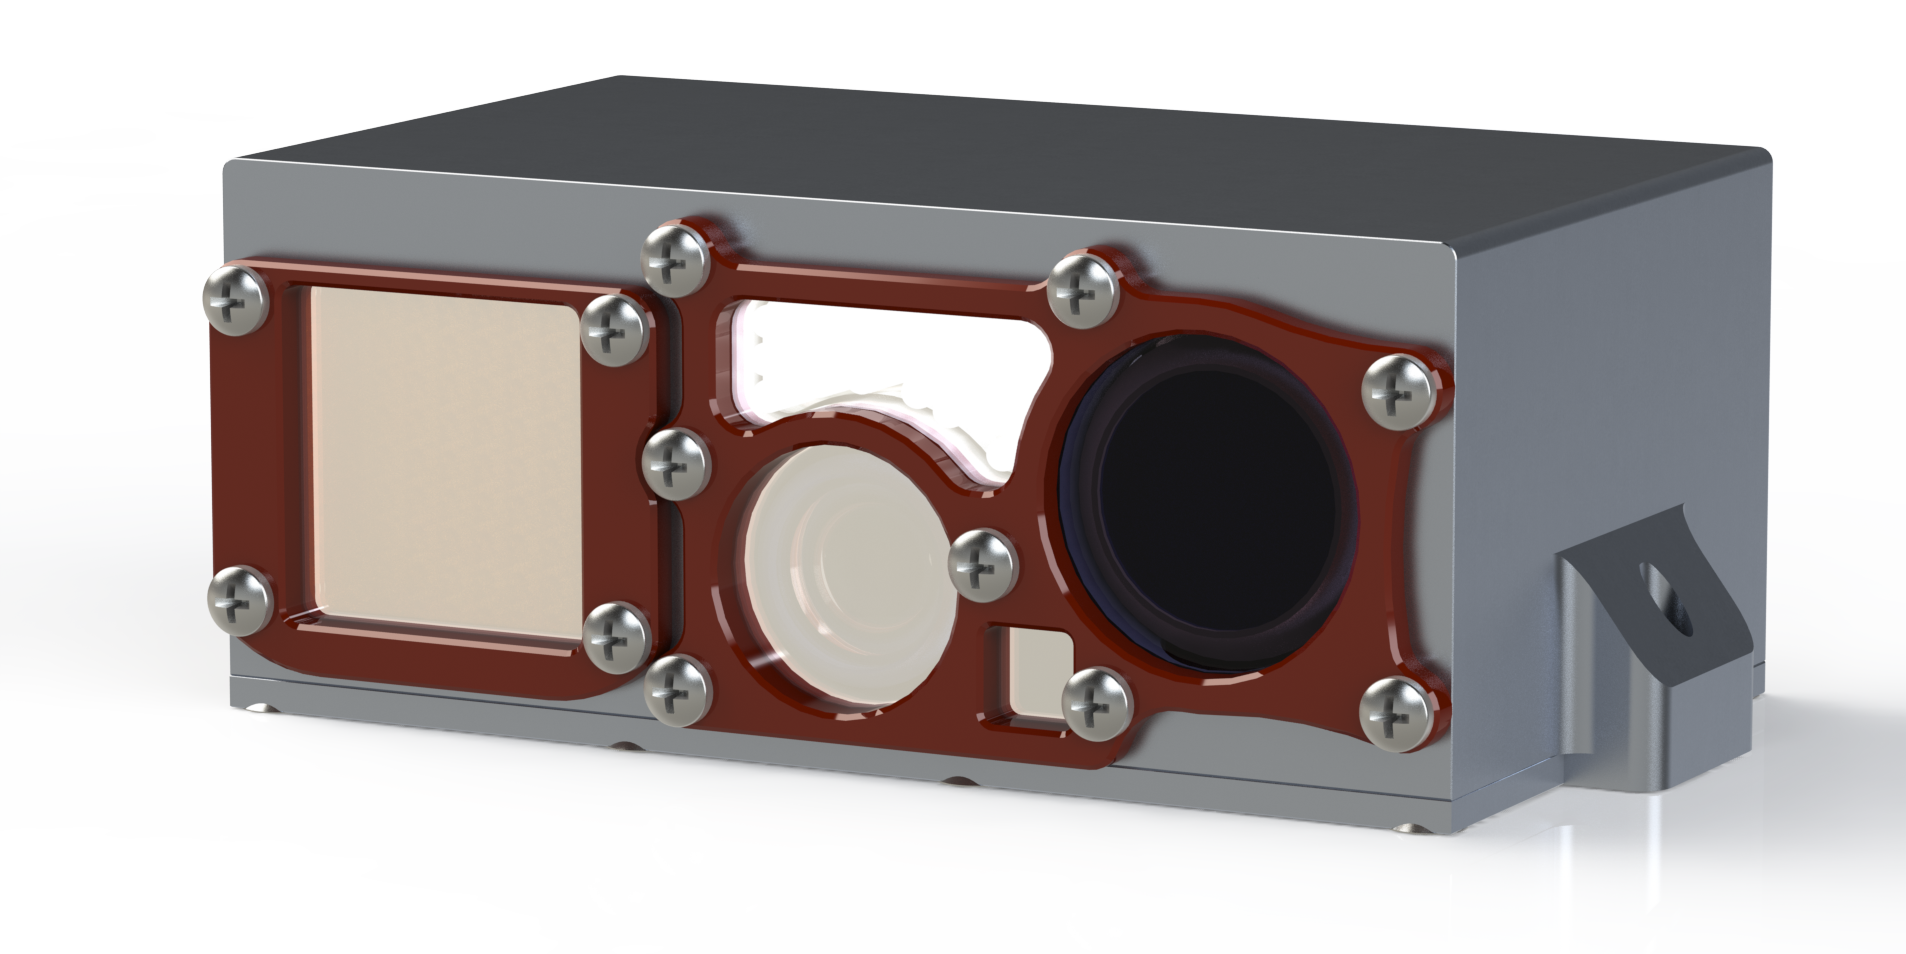
\includegraphics[height=2.6in]{media/VIS-1}
		% \caption{Bezel attachment and release mechanism for a light.}
		\label{VIS 1}
	\end{figure}

% LIGHT FIXTURE
	\section{Light Fixture Release Mechanism Design Challenge}
		\paragraph{Project} Assessment of my design skills and process during interviews for a design firm.
		\paragraph{Goal} Conceptualize and model the bezel attachment and release mechanism for a high-end light fixture and return the design report in 24 hours
		\paragraph{Description} I designed the mechanism to emphasize functionality and discreetness. The bezel features serve a crucial purpose, but should remain unnoticed by working effortlessly and blending into the light's shape. I want them to work easily, so the user forgets they were used. The hinge and clasp must be robust and precise to create a solid seal. The release mechanism's function should be obvious but not obtrusive.  The materials should reflect the quality of the product, and be simple to manufacture.  %improve voice%

	\begin{figure}[H]
		\centering
		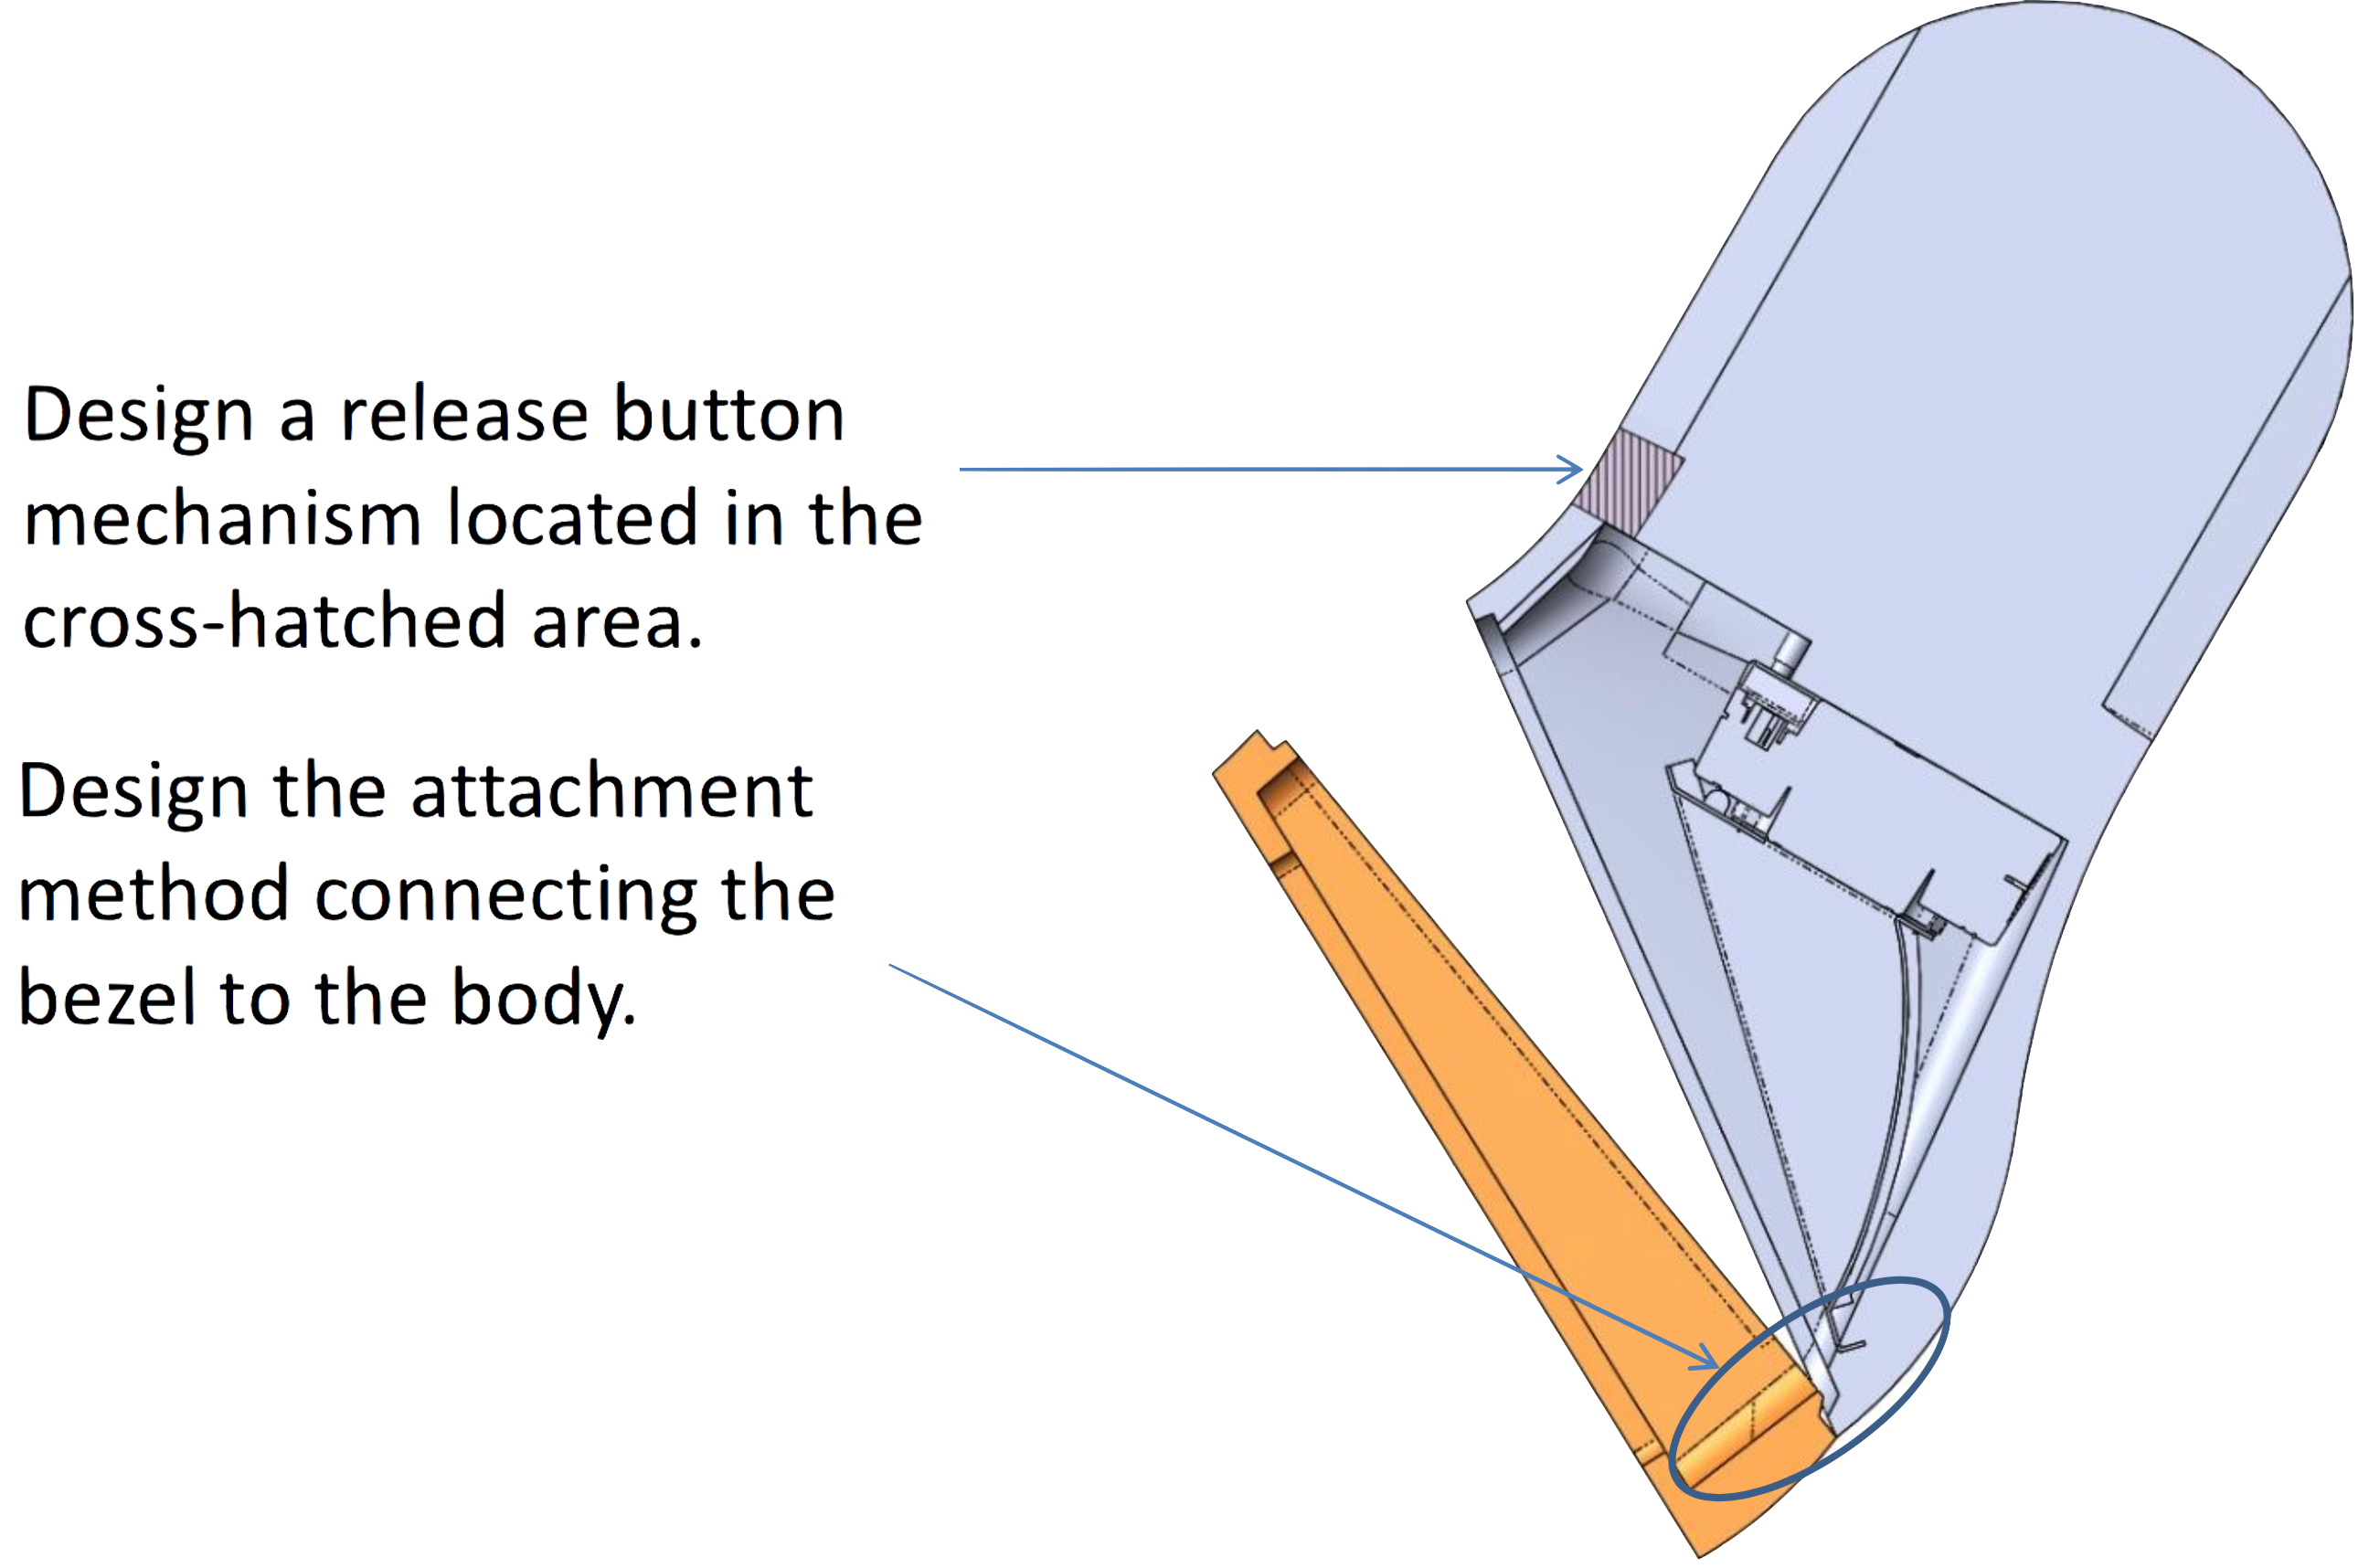
\includegraphics[height=2.6in]{media/inch-task}
		% \caption{Bezel attachment and release mechanism for a light.}
		\label{inch-task}
	\end{figure}

	\clearpage

	\begin{multicols}{2}

		\begin{figure}[H]
			\centering
			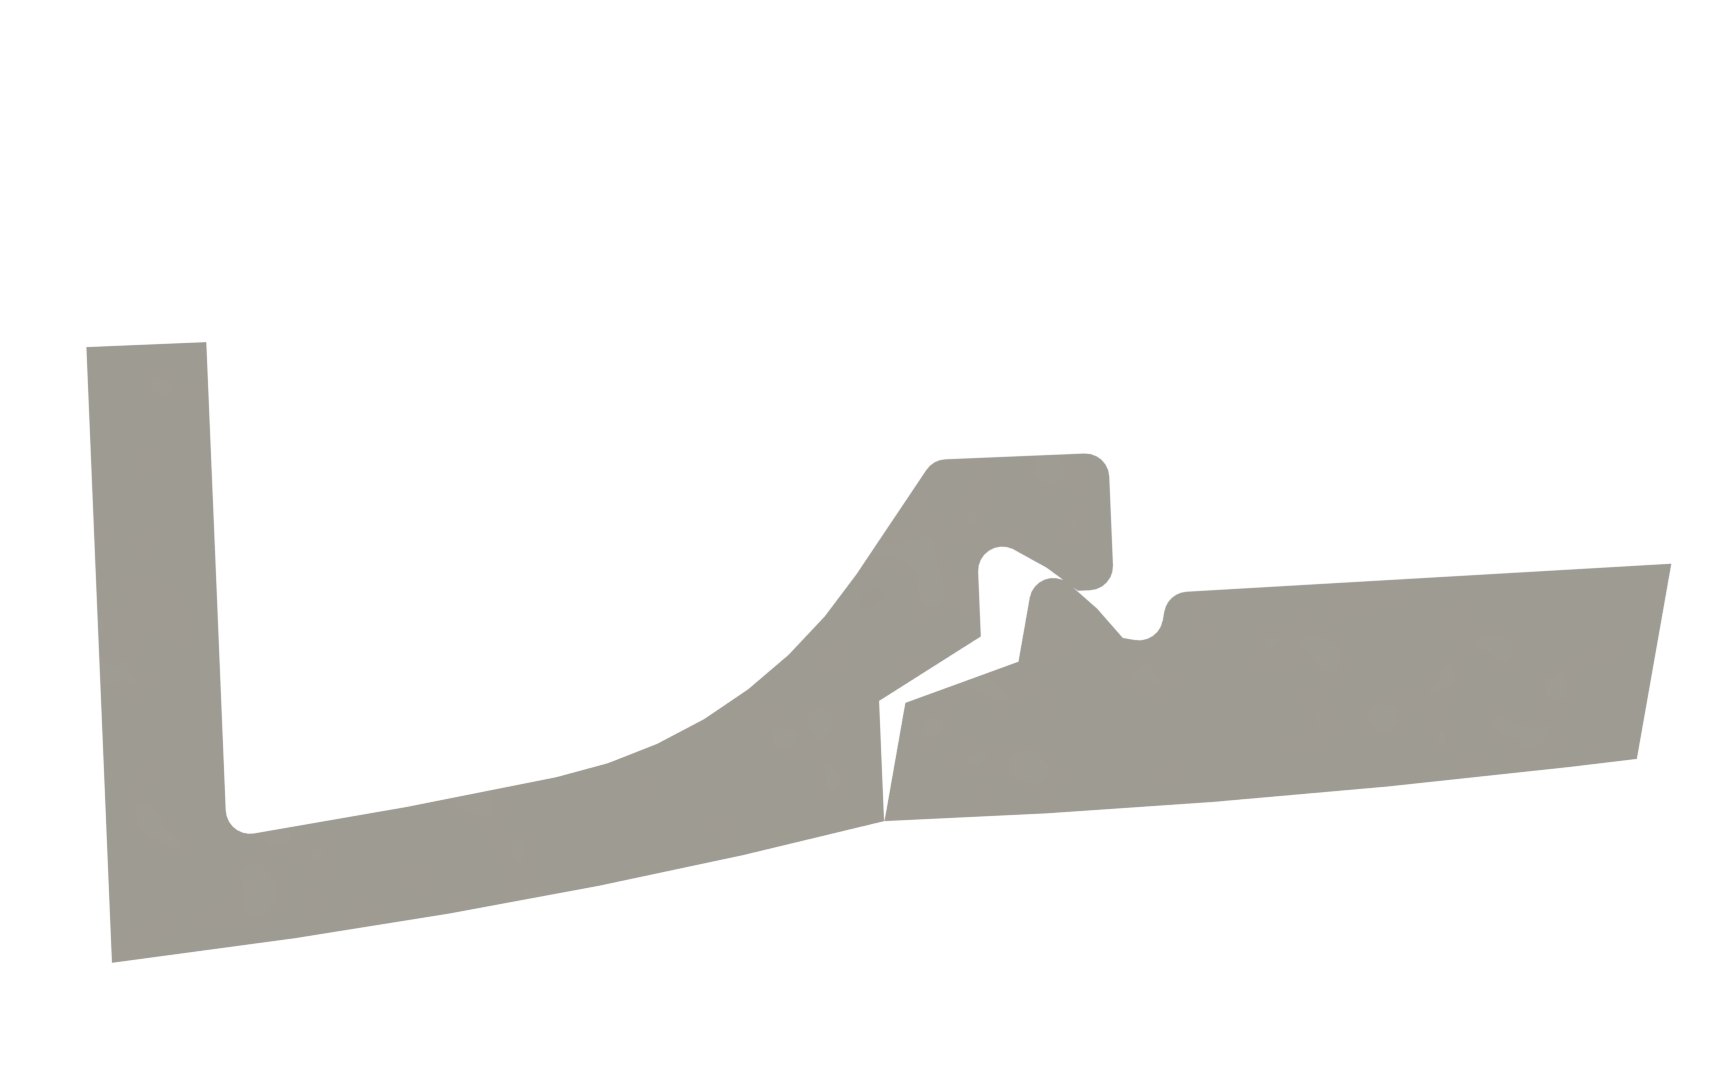
\includegraphics[width=0.5\textwidth]{media/hinge}
			\label{hinge}
		\end{figure}

	\columnbreak

		\begin{figure}[H]
			\centering
			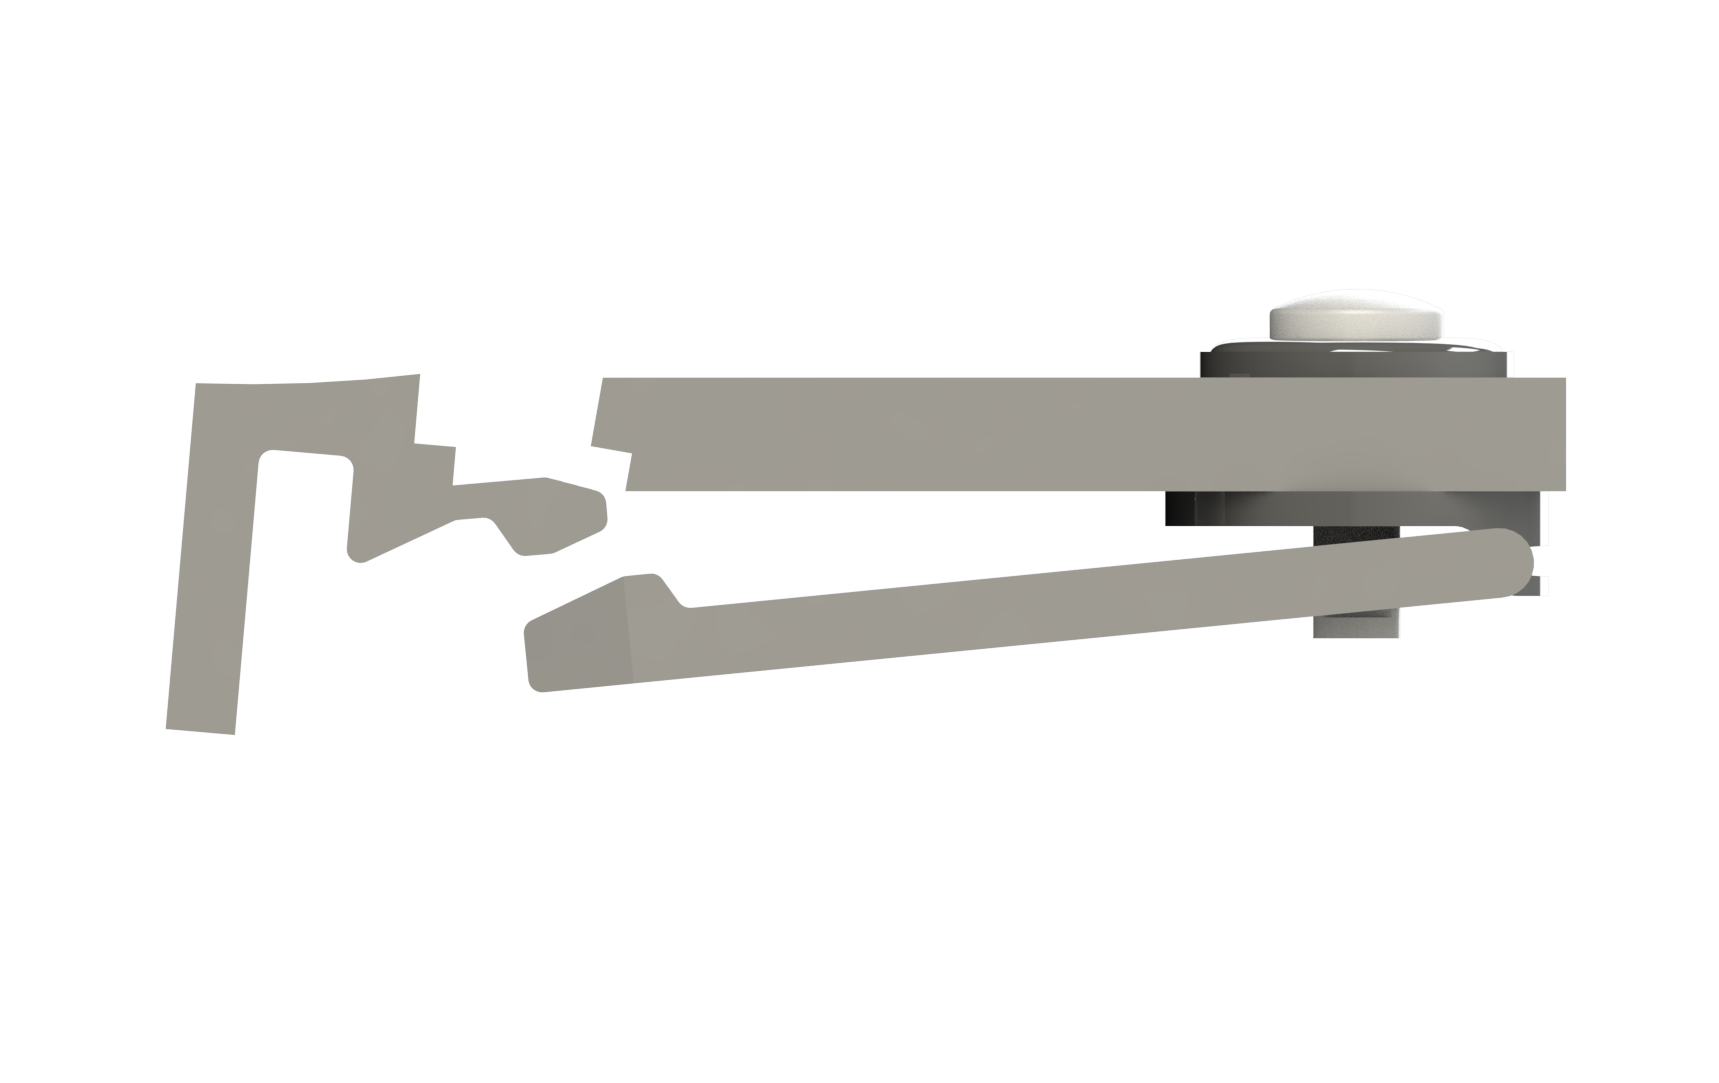
\includegraphics[width=0.5\textwidth]{media/clasp_open}
			\label{clasp_open}
		\end{figure}

	\end{multicols}

	\begin{multicols}{2}

	\paragraph{Hinge}
		The hinge's shape allows the bezel to seat itself on the corner of the fixture and rotate into place.  Once rotated into place, the hinge does not allow the bezel to move outward.

	\columnbreak

	\paragraph{Clasp}
		The clasp is a wedge that applies a radial force on the body to create a snug fit against the inside of the fixture.  To secure it in the axial direction, the button lever hooks the clasp to lock it into place.
	
	\end{multicols}

		\begin{figure}[H]
			\centering
			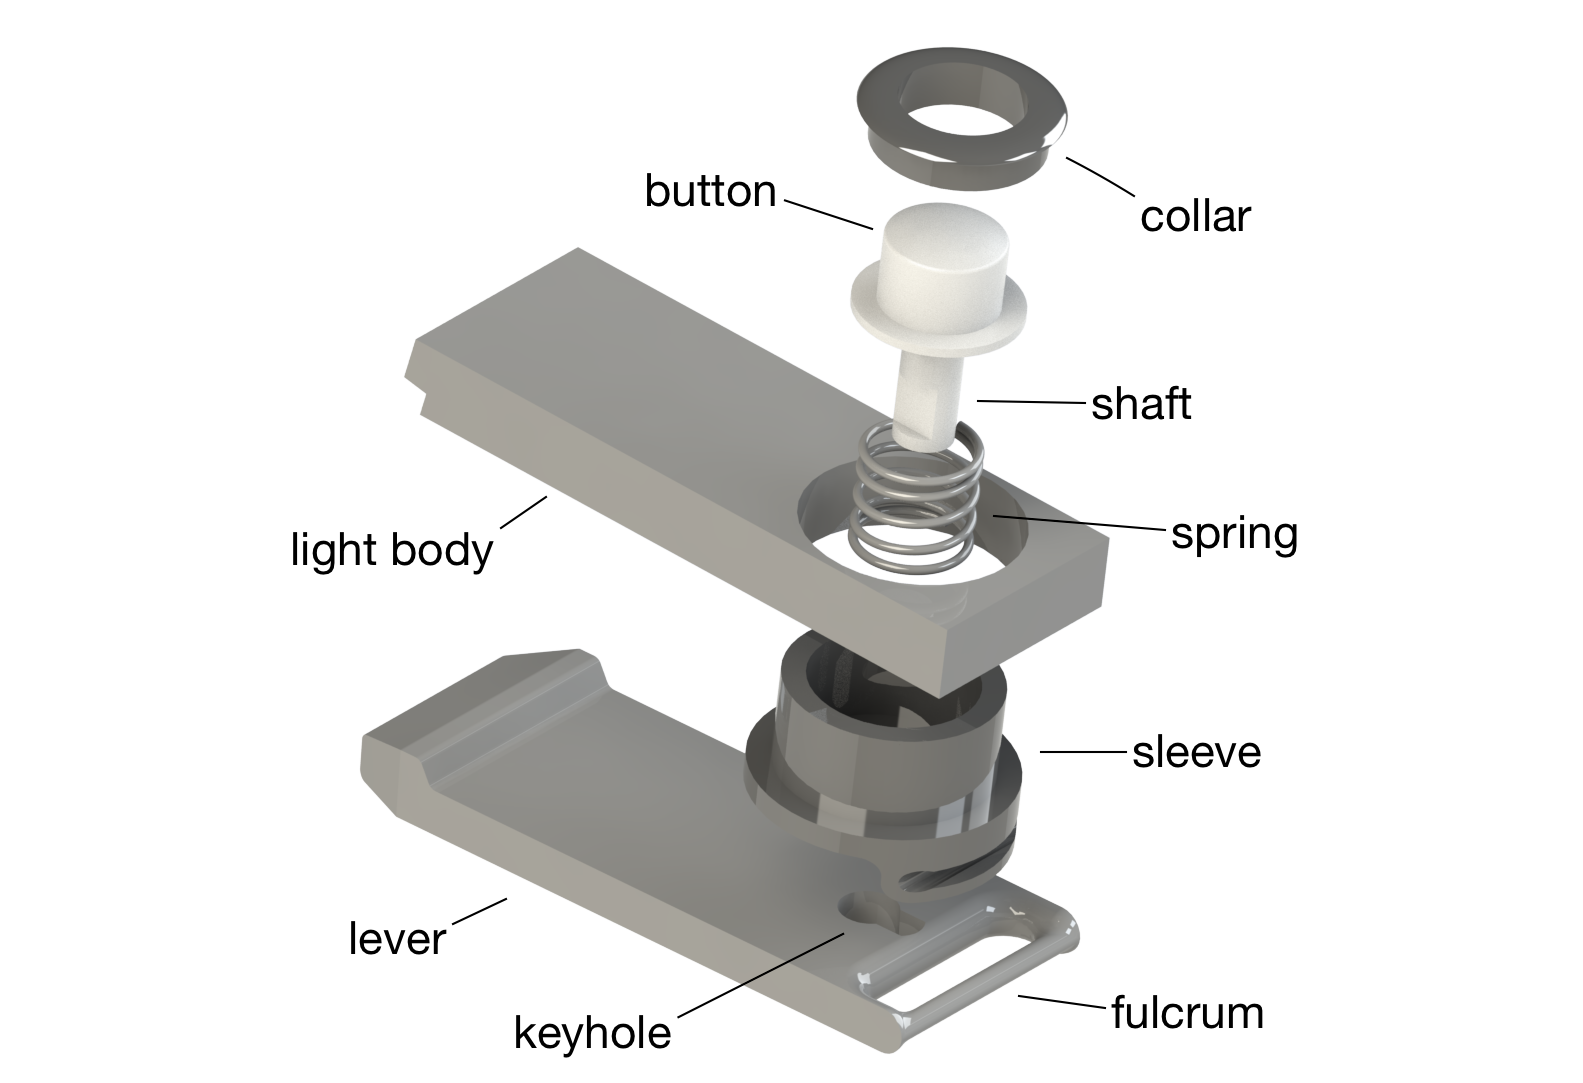
\includegraphics[width=0.75\textwidth]{media/button_exploded}
			\label{button_open}
		\end{figure}

	\paragraph{Button}
		The button releases the bezel when pushed. It does not deliver much force, because it only opens the clasp, rather than push the bezel out.  It uses a lever for mechanical advantage, requiring less travel when pushed. A keyhole in the lever accepts the notched shaft and allows the lever to slide forward as its fulcrum snaps into the back of the sleeve.  The flange on the shaft locks the button into the keyhole while the spring keeps it extended.

	

		\clearpage

% ENCLOSURE
	\section{Wearable Electronics Enclosure Prototype}
		\paragraph{Project} 3D-printed Enclosure Prototype for a Wearable Mixed-Signal Sensor Circuit for the McGill University \href{http://www.ece.mcgill.ca/~vchoda/Research.htm}{Sensor Microsystems Laboratory}
		\paragraph{Goal} Enclose a small sensor circuit board with a hermetic seal and diaphragm to allow the measurement of pressure change under changing loads
		\paragraph{Description} In order to pitch the device to a potential customer, my client needed a prototype enclosure with enough fidelity to sell the customer on the functionality of the product.  The project was given to me on short notice over a weekend, so I completed it in one day.

	\begin{figure}[H]
		\centering
		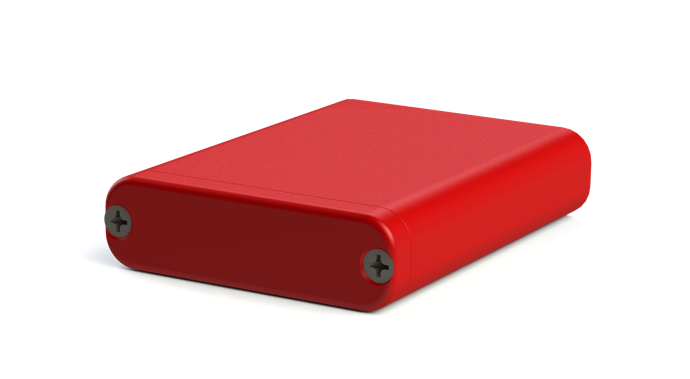
\includegraphics[height=2.75in]{media/enclosure_render}
		\label{enclosure_render}
	\end{figure}

	\begin{figure}[H]
		\centering
		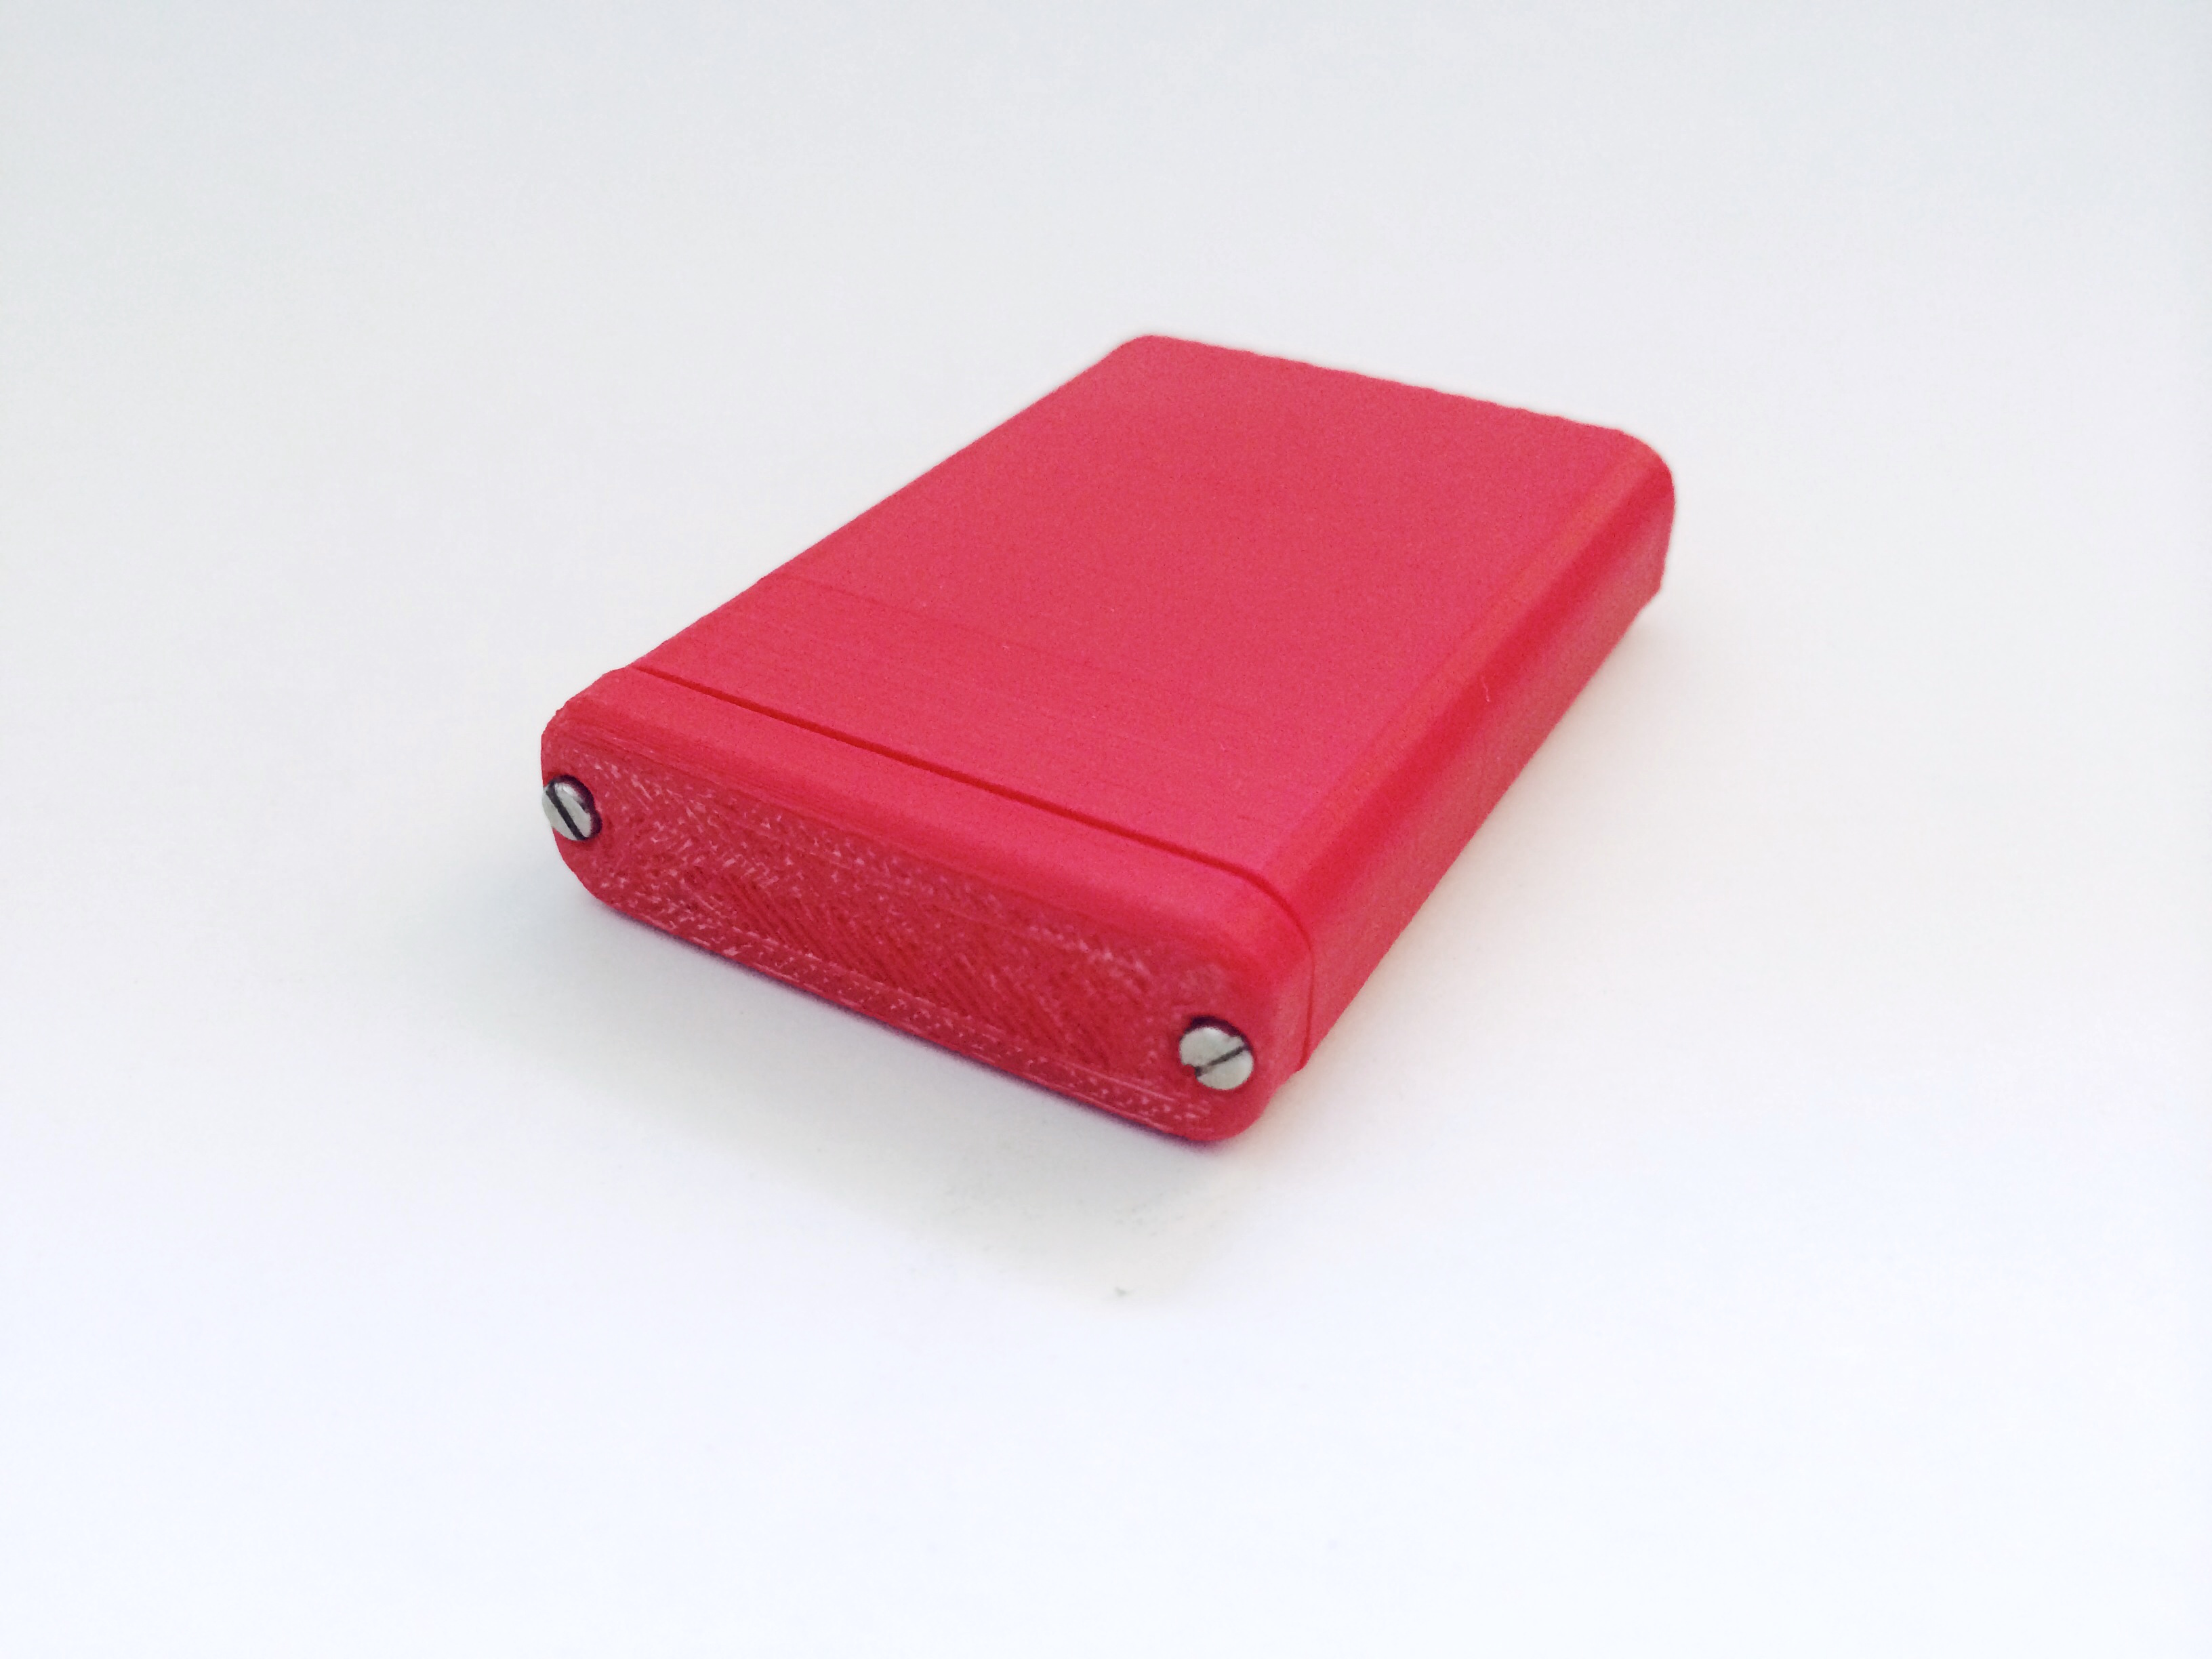
\includegraphics[height=4in]{media/enclosure_closed}
		\caption{Electronics enclosure sealed}
		\label{enclosure_sealed}
	\end{figure}

	The 3D printed prototype encapsulates a small circuit board and battery, with a "hermetic" o-ring seal, and fastened with two screws.  I printed it with ABS on a Makerbot Replicator 2X in one iteration.

	\begin{figure}[H]
		\centering
		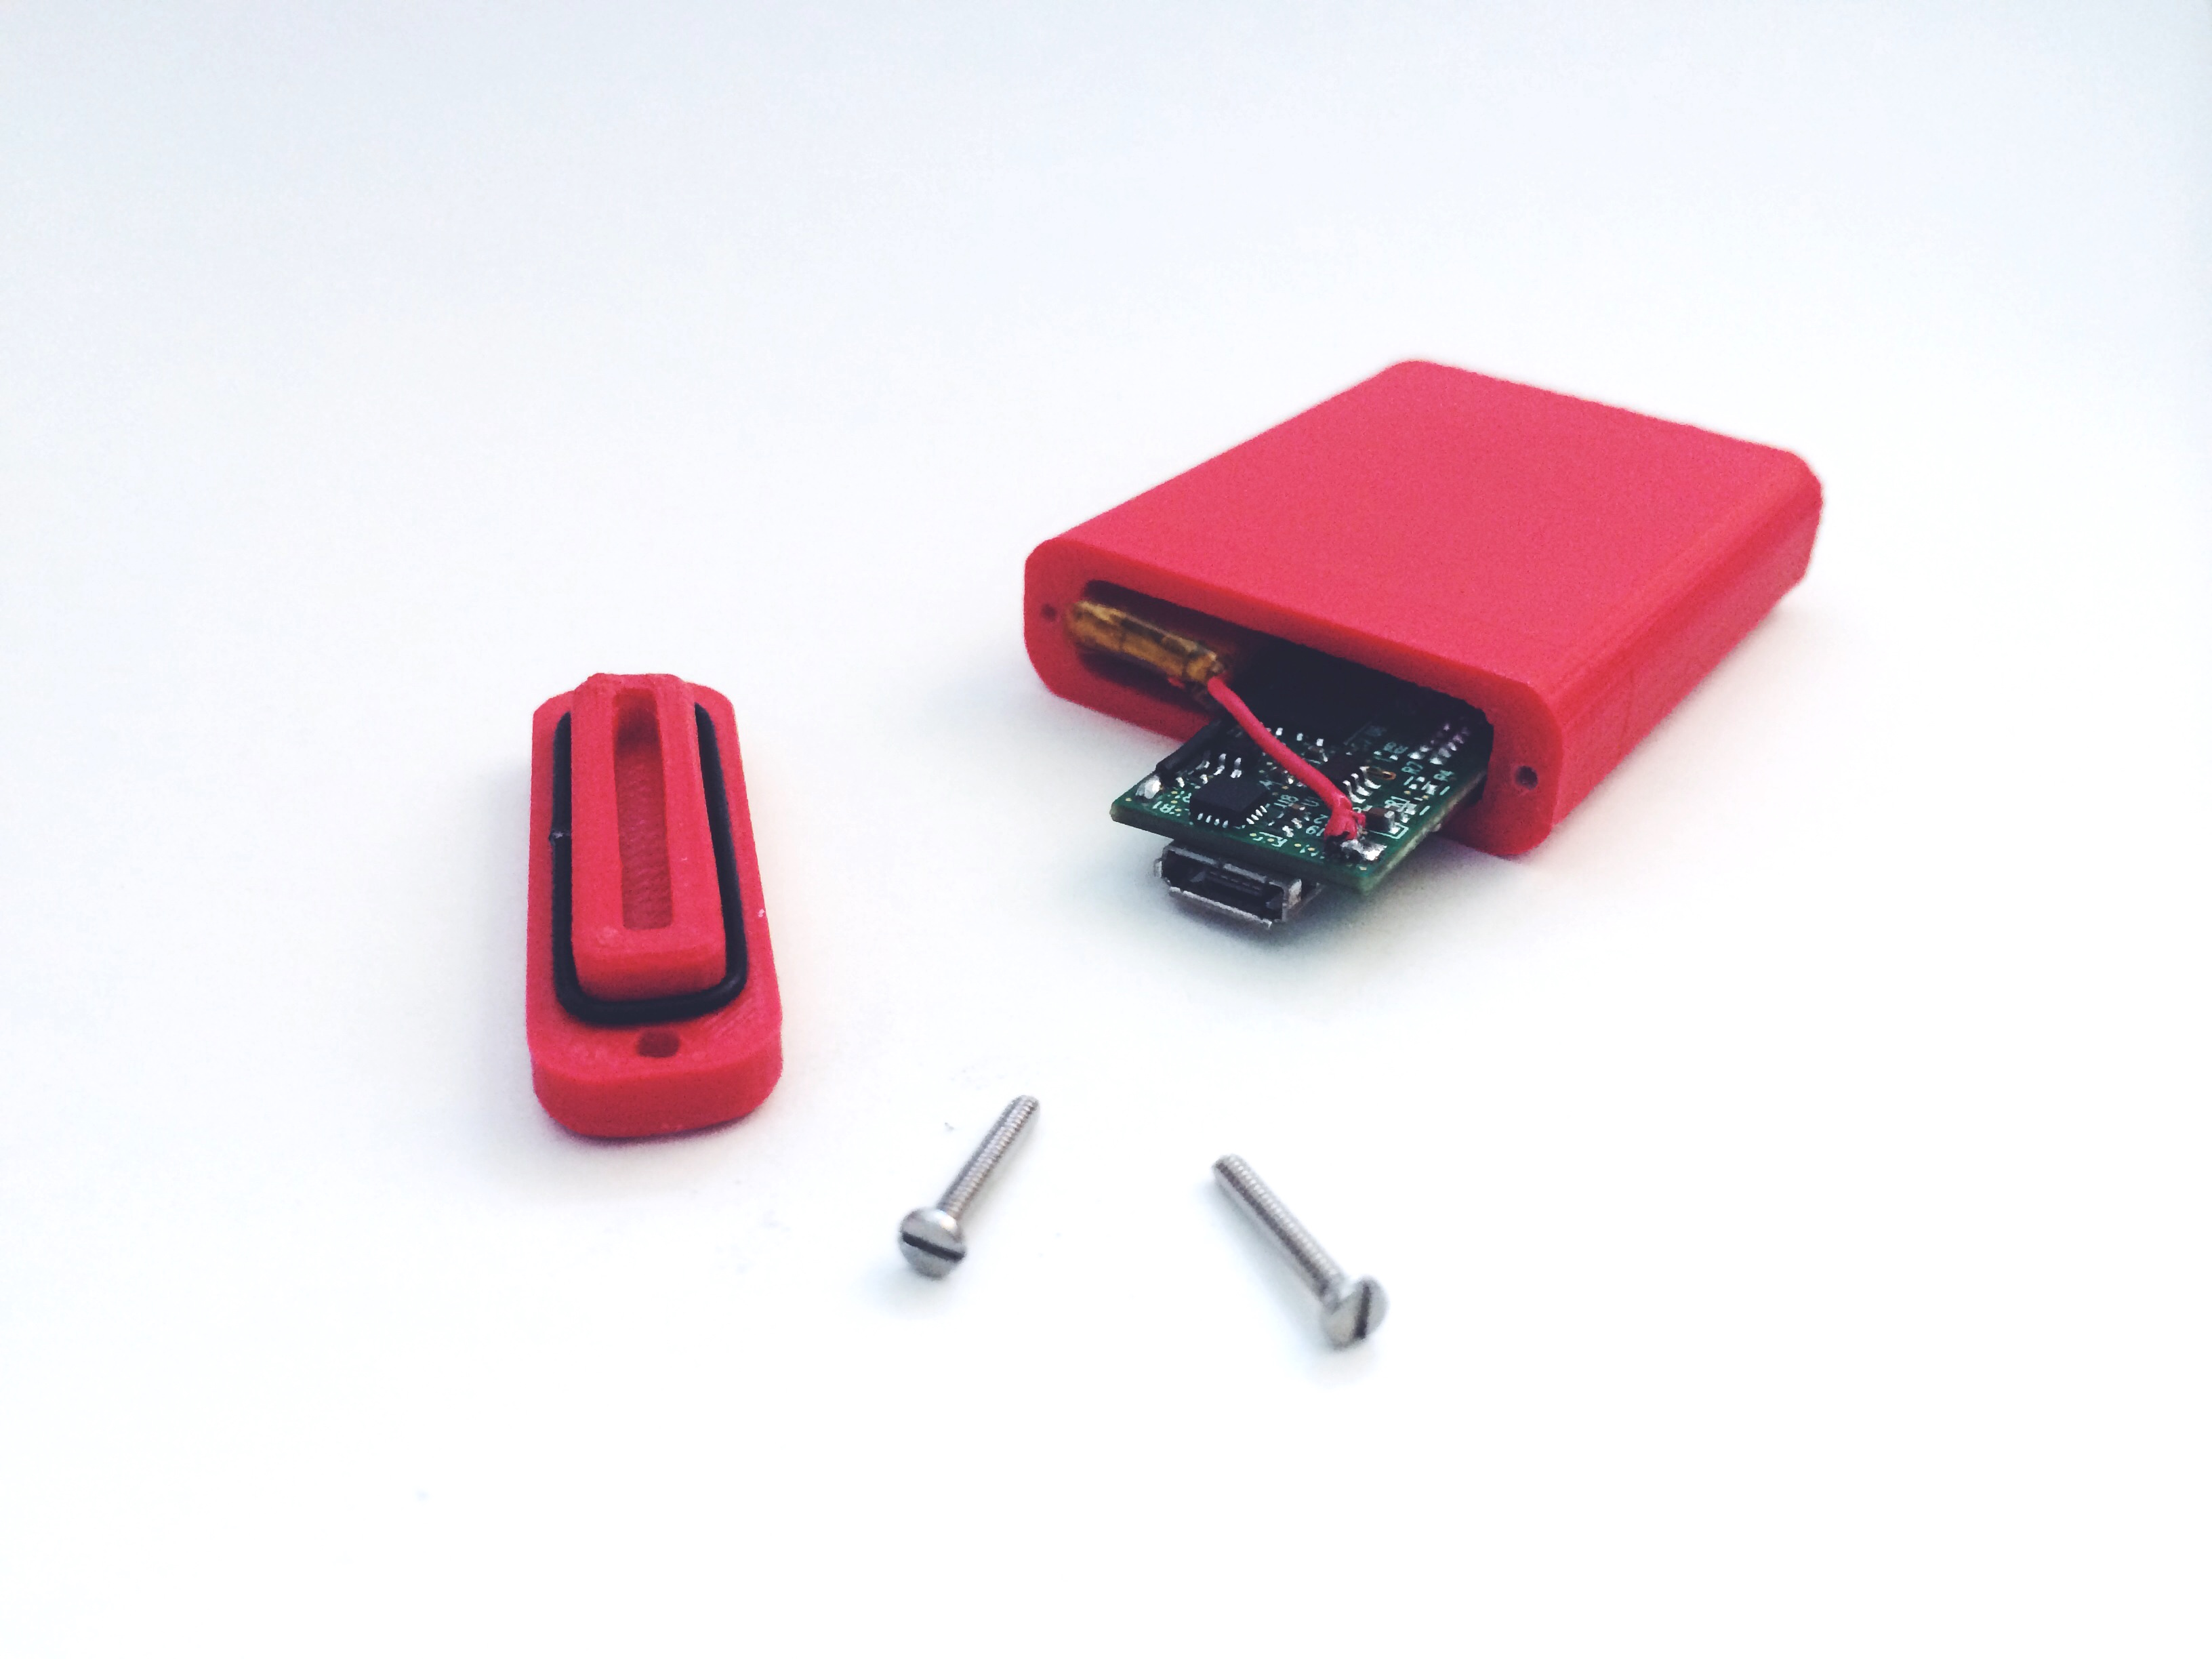
\includegraphics[height=4in]{media/enclosure_open}
		\caption{Electronics enclosure open}
		\label{enclosure_open}
	\end{figure}

	The enclosure is a simple container and cap design, with one wall of the container made thin (1.0mm thick) to create a flexible membrane that deforms under load. The sensor inside detects the pressure change due to volume change.

% VF SHOE
	\section{Variable-Friction Shoe Surface Mechanism}
		\paragraph{Project} Research for Professor~\href{http://www.cim.mcgill.ca/~jer/}{Jeremy Cooperstock} of~ \href{http://www.cim.mcgill.ca/sre}{The Shared Reality Lab} - McGill Centre for Intelligent Machines
		\paragraph{Goal} Design, manufacture, assemble, and demonstrate a mechanism to fit in the sole of a shoe that can adjust the coefficient of friction between the shoe and the floor surface.
		\paragraph{Description} McGill University's Shared Reality Lab studies methods of varying friction during natural walking for its applications in simulated environments and needed a mechanism to actively adjust friction. In seven months I created from scratch a device that replaces the heel of a boot and varies friction to simulate walking surfaces from ice to concrete.  
		% Creating the concept involved choosing a method of deployment, calculating geometry and dynamics, analyzing stresses, designing a layout to fit in the envelope, CAD modeling the device, and researching components and materials for manufacturing.  I spent three months in the machine shop manufacturing, assembling, and testing the mechanical components to ensure an operational device and another month wiring the motor circuit and coding the controller.  I tested the device to confirm the full range of friction adjustment and it was immediately put to use by the Shared Reality Lab for research. %review. explain why? explain its heel portion%

		A full design report can be found at~\href{http://michaelelliotking.com/report}{michaelelliotking.com/report}.
		\begin{figure}[H]
			\centering
			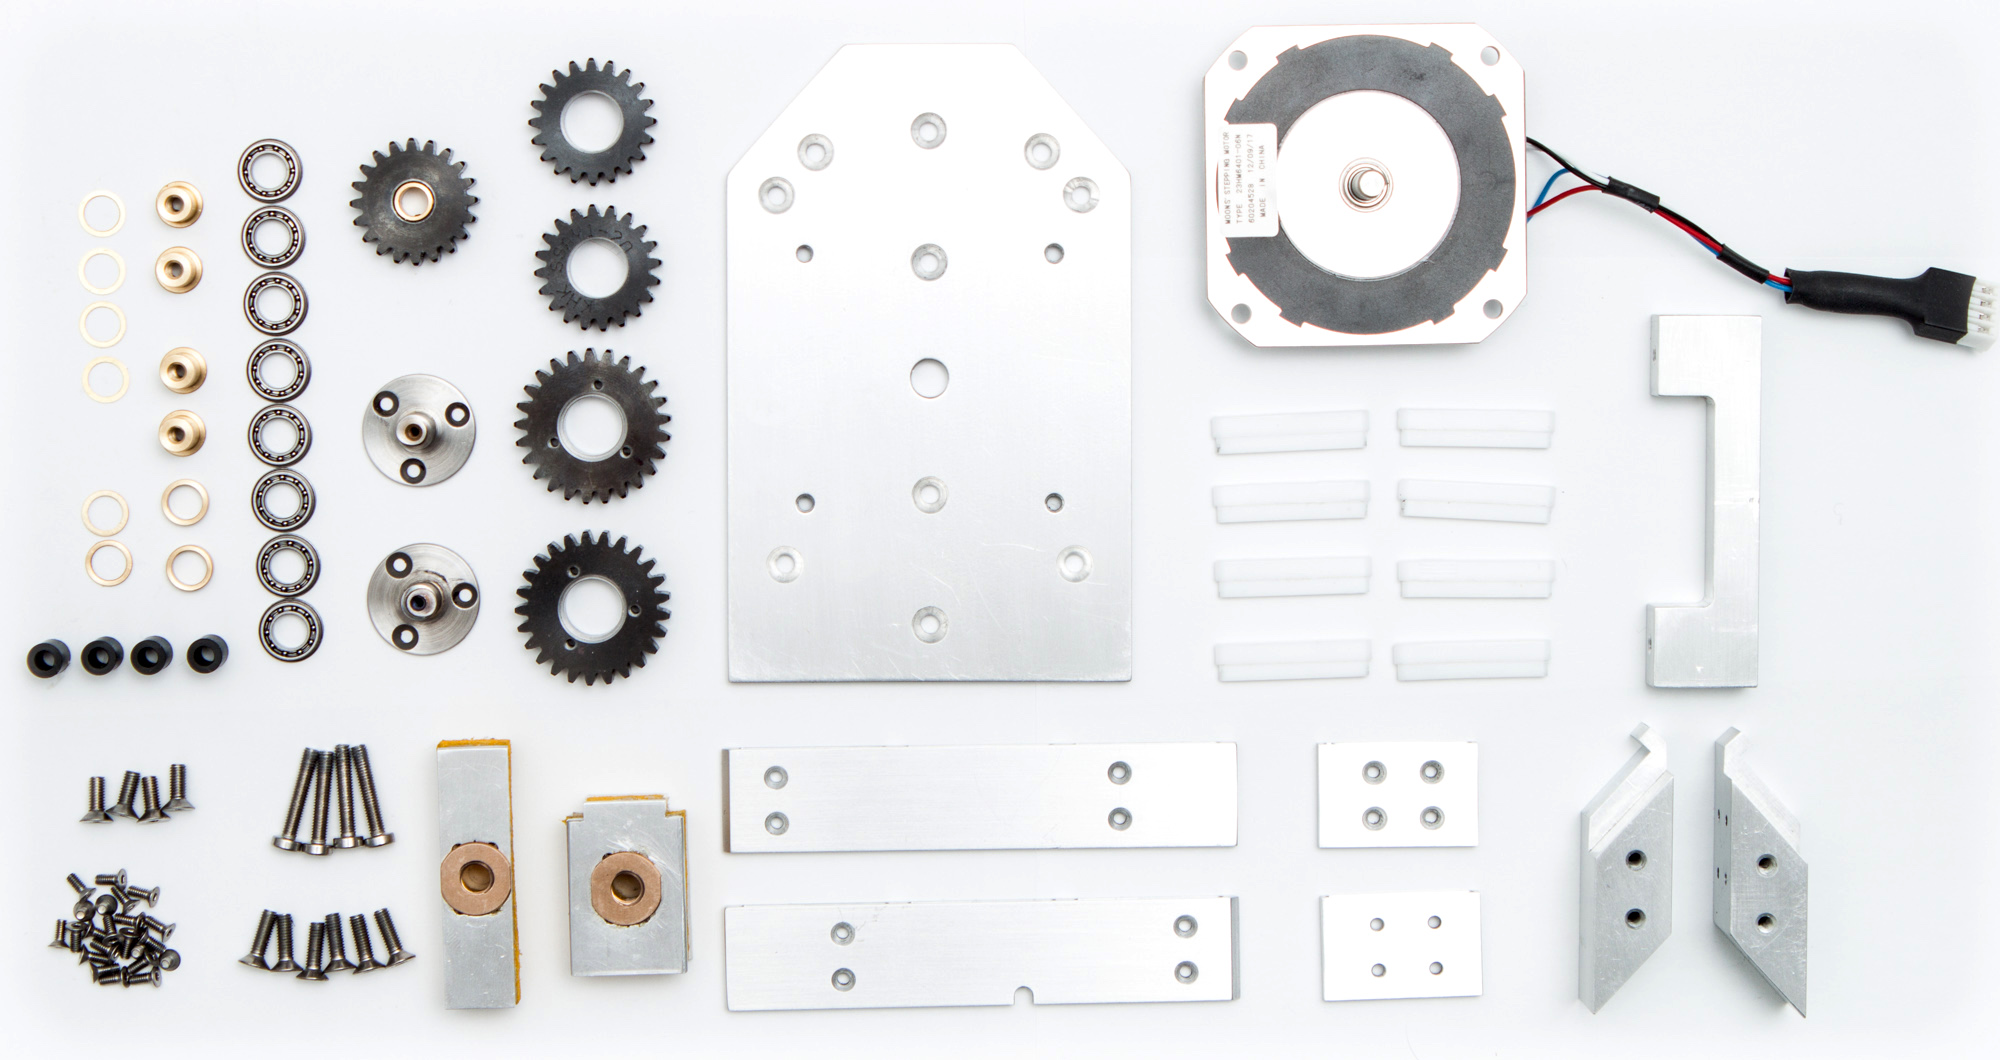
\includegraphics[height=2.75in]{media/shoe_components}
			% \caption{The underside of the mechanism, visible when replaced for the heel of a shoe}
			\label{components}
		\end{figure}

		\begin{figure}[H]
			\centering
			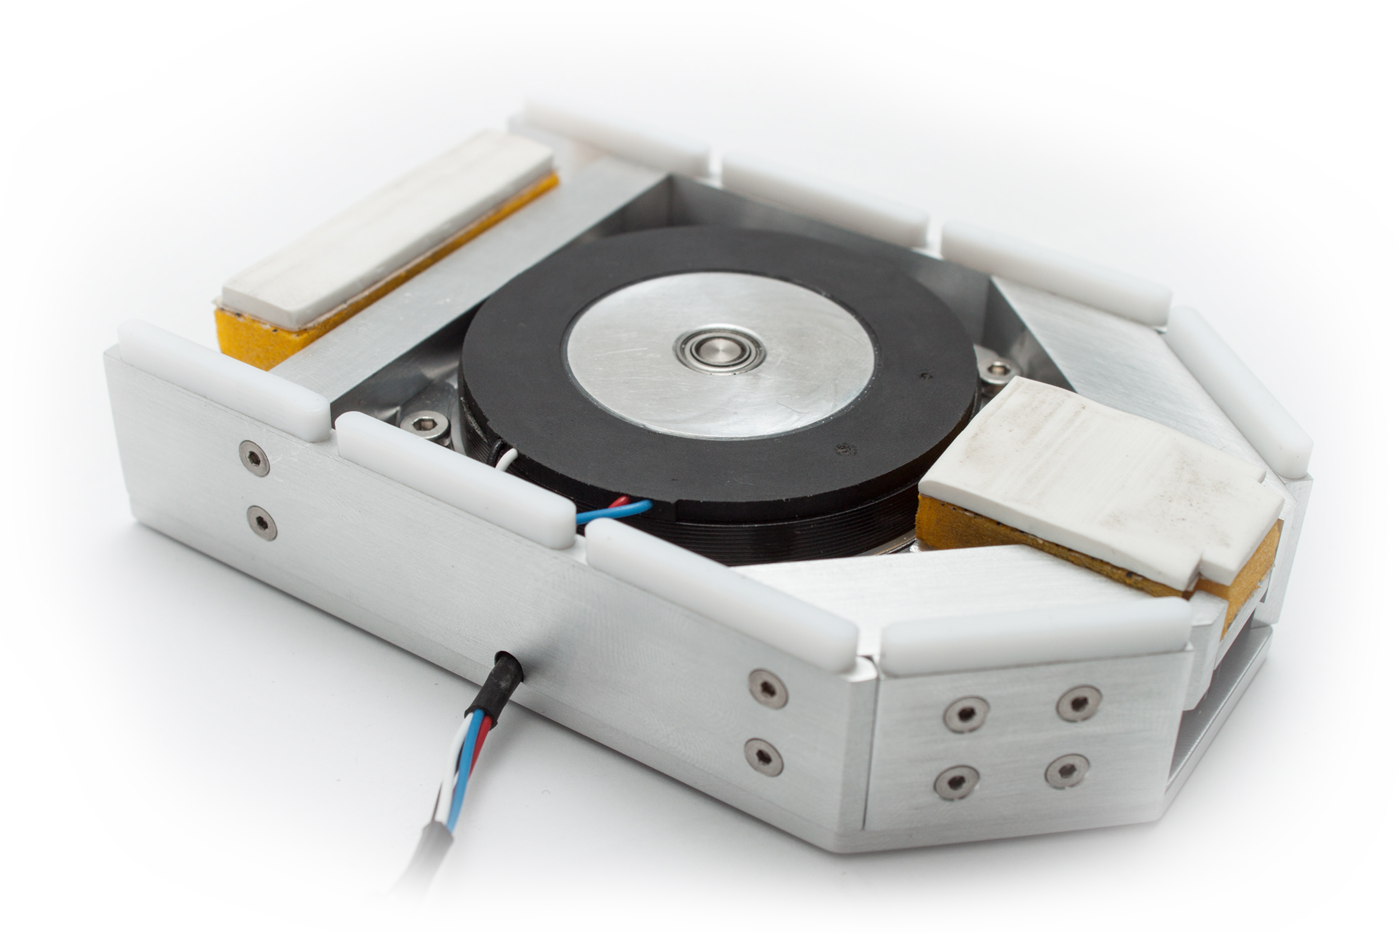
\includegraphics[height=4in]{media/shoe_prototype}
			\caption{The underside of the mechanism, visible when replaced for the heel of a shoe}
			\label{overview}
		\end{figure}

		I simulated a range of surfaces---from ice to concrete---by varying the device's coefficient of friction using the combination of adjustable, deformable, high-friction brake pads and rigid, static, low-friction Teflon rails.  The height of the deformable brakes is adjusted to control the weight distribution between them and the Teflon rails during walking. And because friction force is proportional to normal force---on both the brakes and rails---the device's net coefficient of friction changes with the brakes' height. 

		\begin{figure}[H]
			\centering
			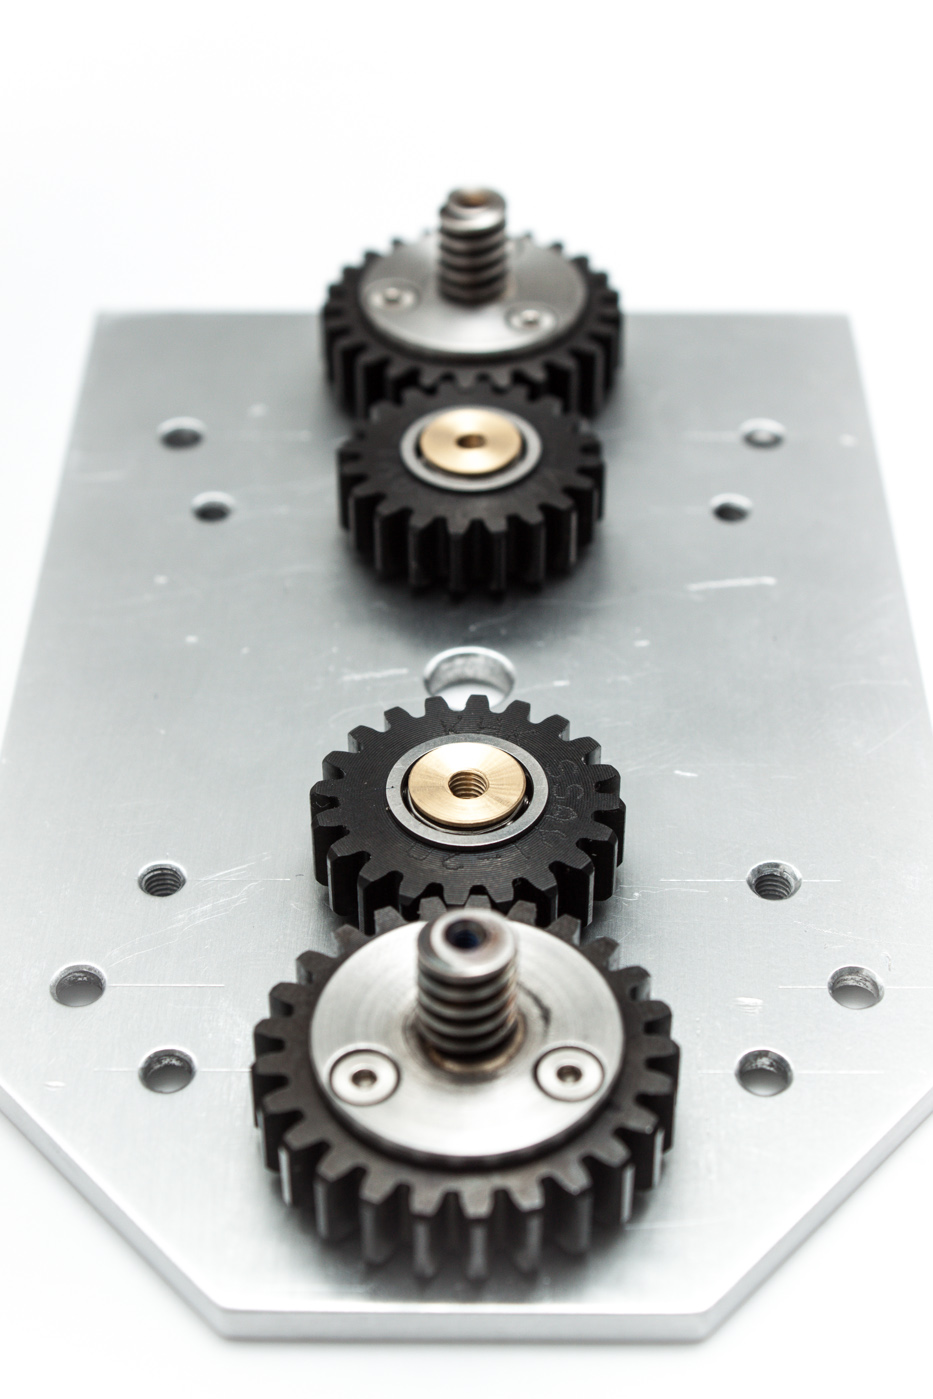
\includegraphics[height=4in]{media/gears_attached}
			\caption{The drive train before the motor is attached in the center (and covers the inner gears)}
			\label{drive}
		\end{figure}

		A central stepper motor drives the gears and a lead screw threaded into each brake changes the height of the braking surface.  I developed the drive system myself, and every component except the gears and bearings were machined in-house from aluminum, stainless, and brass.

		\begin{figure}[H]
			\centering
			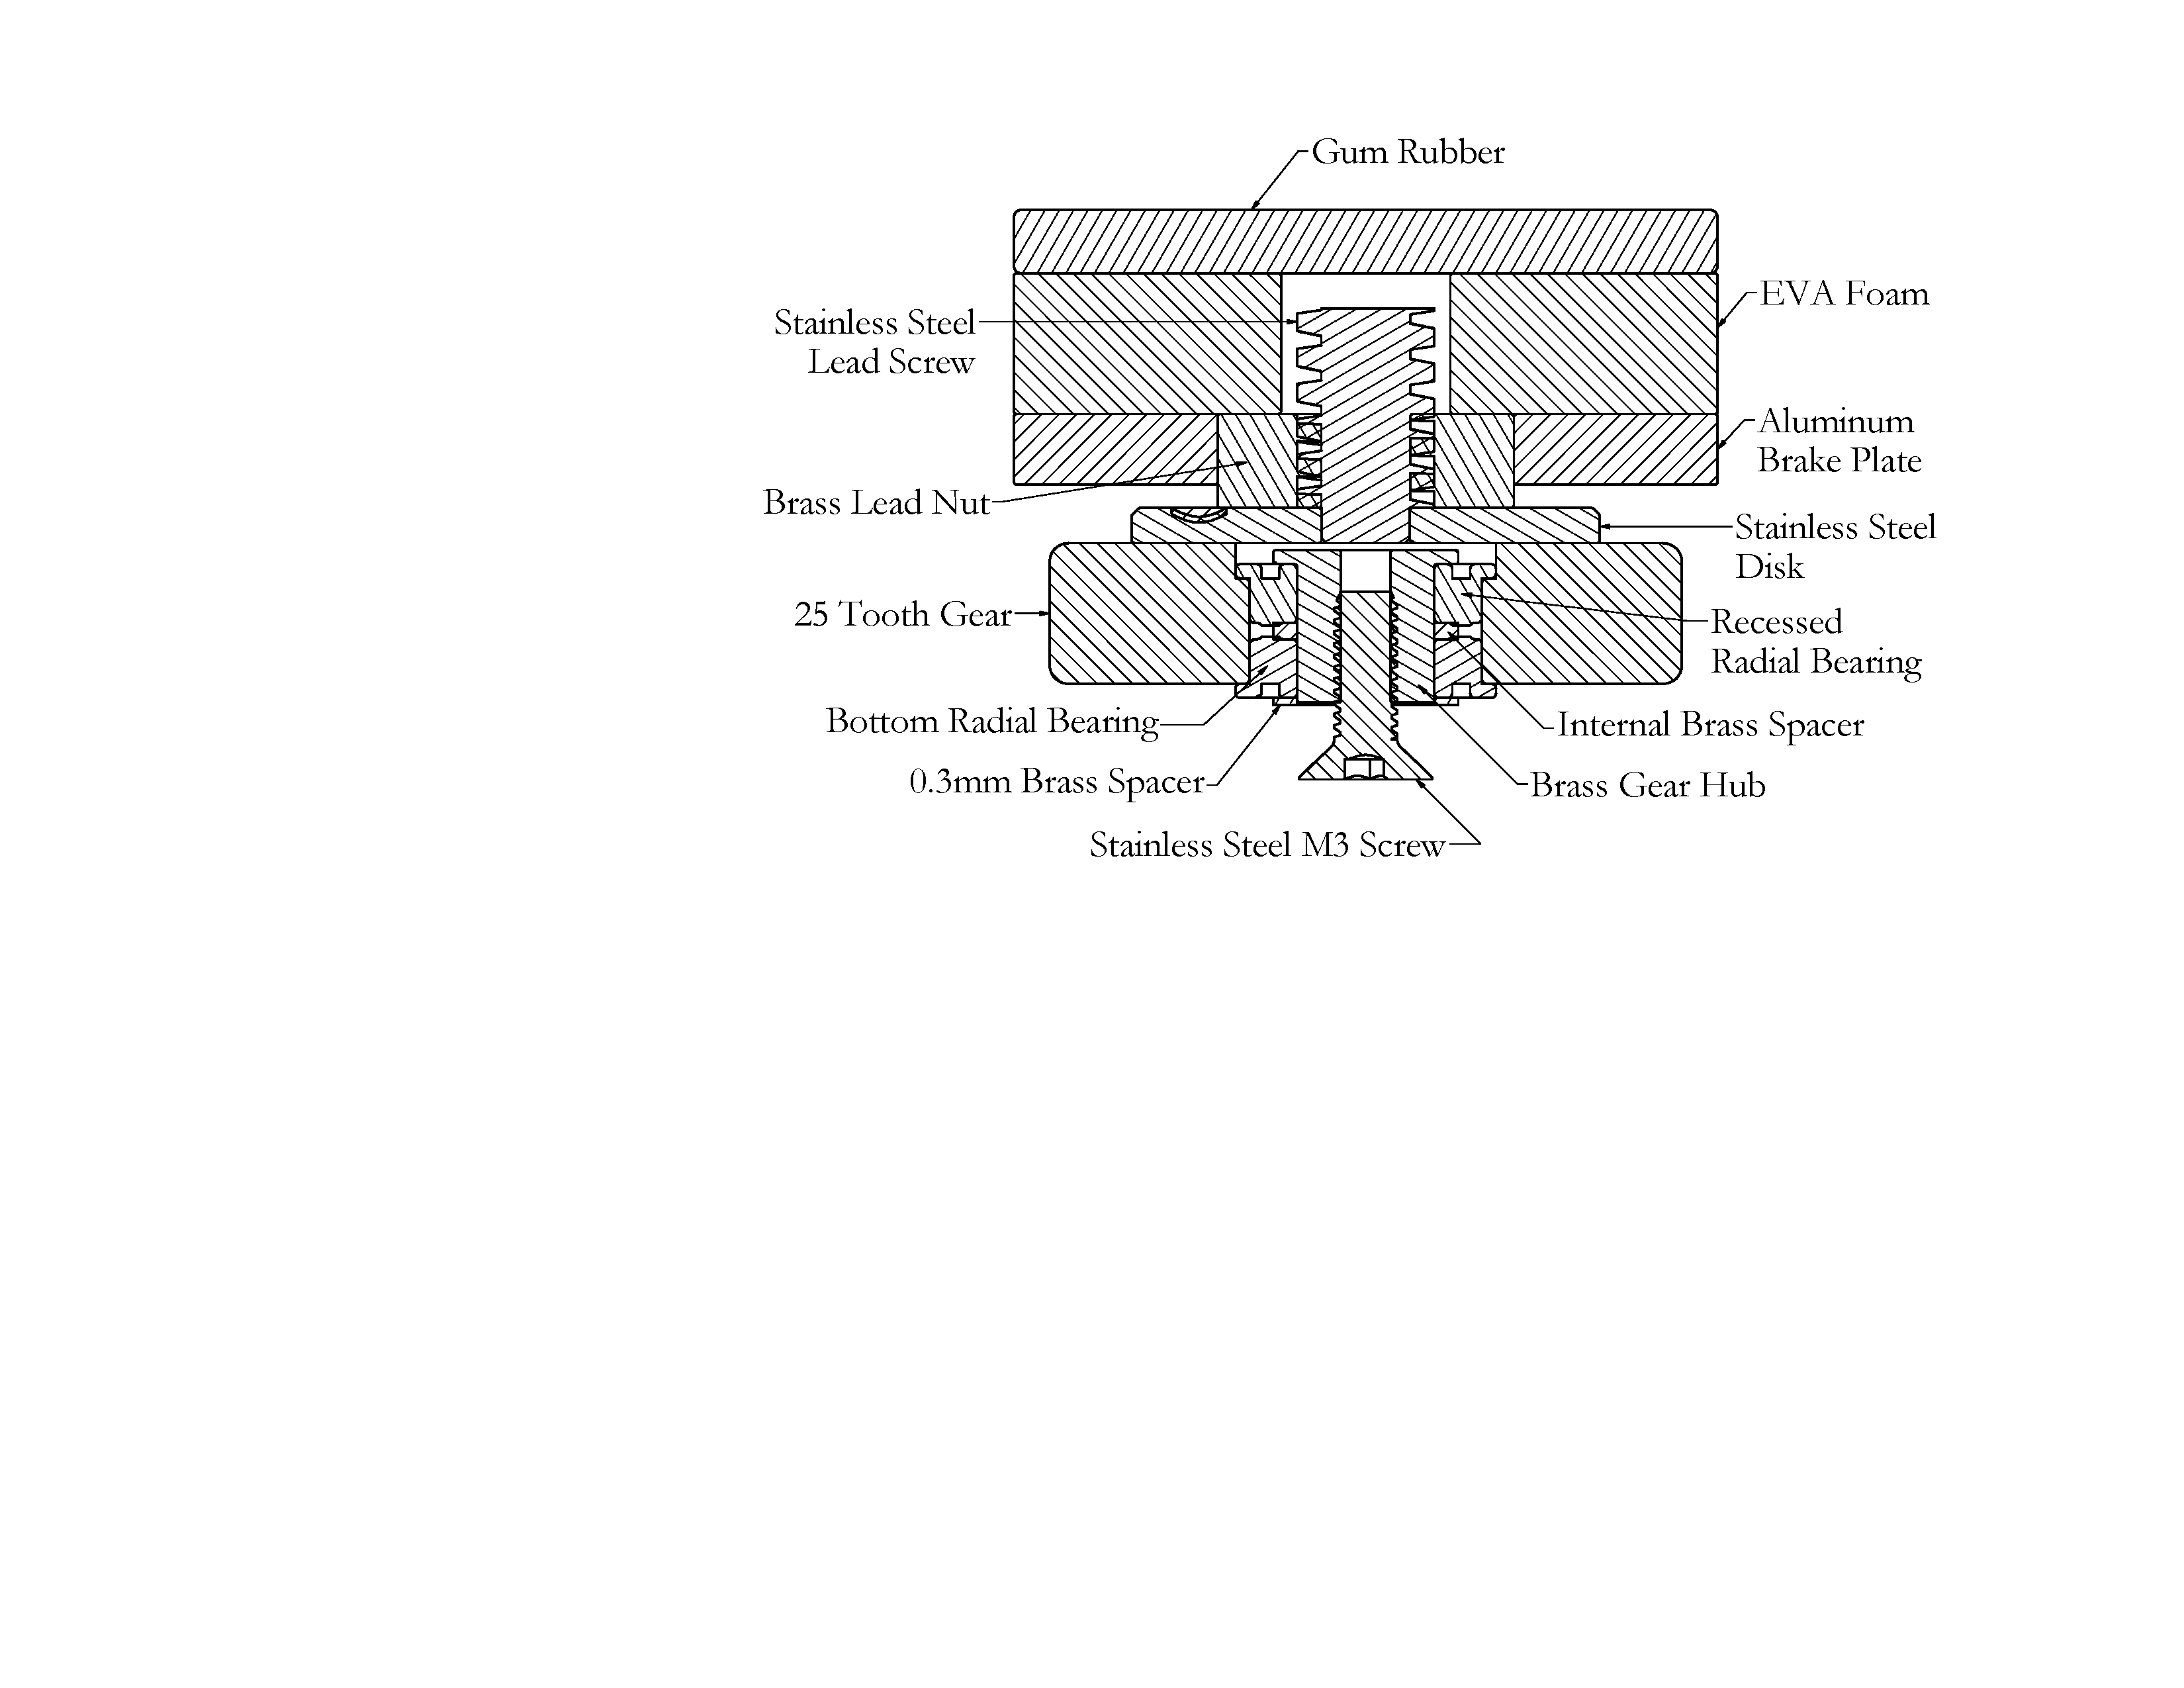
\includegraphics[height=4in]{media/cutaway}
			\caption{Cut-away view of a brake assembly}
			\label{cutaway}
		\end{figure}

		The lead screw rotates with the gear, which is sandwiched between bearings and spacers, and threaded into the lead nut embedded in the aluminum brake plate.  The plate, a piece of EVA foam for elasticity, and a strip of rubber for high friction form each brake.  The stepper motor's precision and the gears' ratio allow precise translations of the brake pads as small as a tenth of a millimeter, which is needed to achieve specific coefficients of friction.

\clearpage

% AUV
	\section{Autonomous Underwater Vehicle}
		\paragraph{Project} Autonomous Underwater Vehicle for the \href{http://www.mcgillrobotics.com}{McGill Robotics Design Team}
		\paragraph{Goal} Design, analyze, manufacture, implement and test an A.U.V. to compete in the \href{http://www.robosub.org}{AUVSI Robosub Competition} in San Diego, CA in July 2014.
		\paragraph{Description} Two months are used to research existing teams and industry designs, develop concepts, and evaluate them based on cost, simplicity, and manufacturability.  Another two months are spent designing, CADing, and running FEA, to prepare for purchasing.  Machine drawings are made and materials are ordered over the next month.  Following this, one month is spent on machining, printing, and manufacturing, and less than a month assembling the components.  The next four months are left for unit testing, dry testing, and finally wet testing.  This period is also left open for any necessary redesign and manufacturing that will inevitably take place.  The vehicle must be ready for competition in June to allow for shipping and travel to San Diego.
		In the next few pages, some of the major components that were CADed are shown in more detail.

	\begin{samepage}
		\begin{figure}[H]
			\centering
			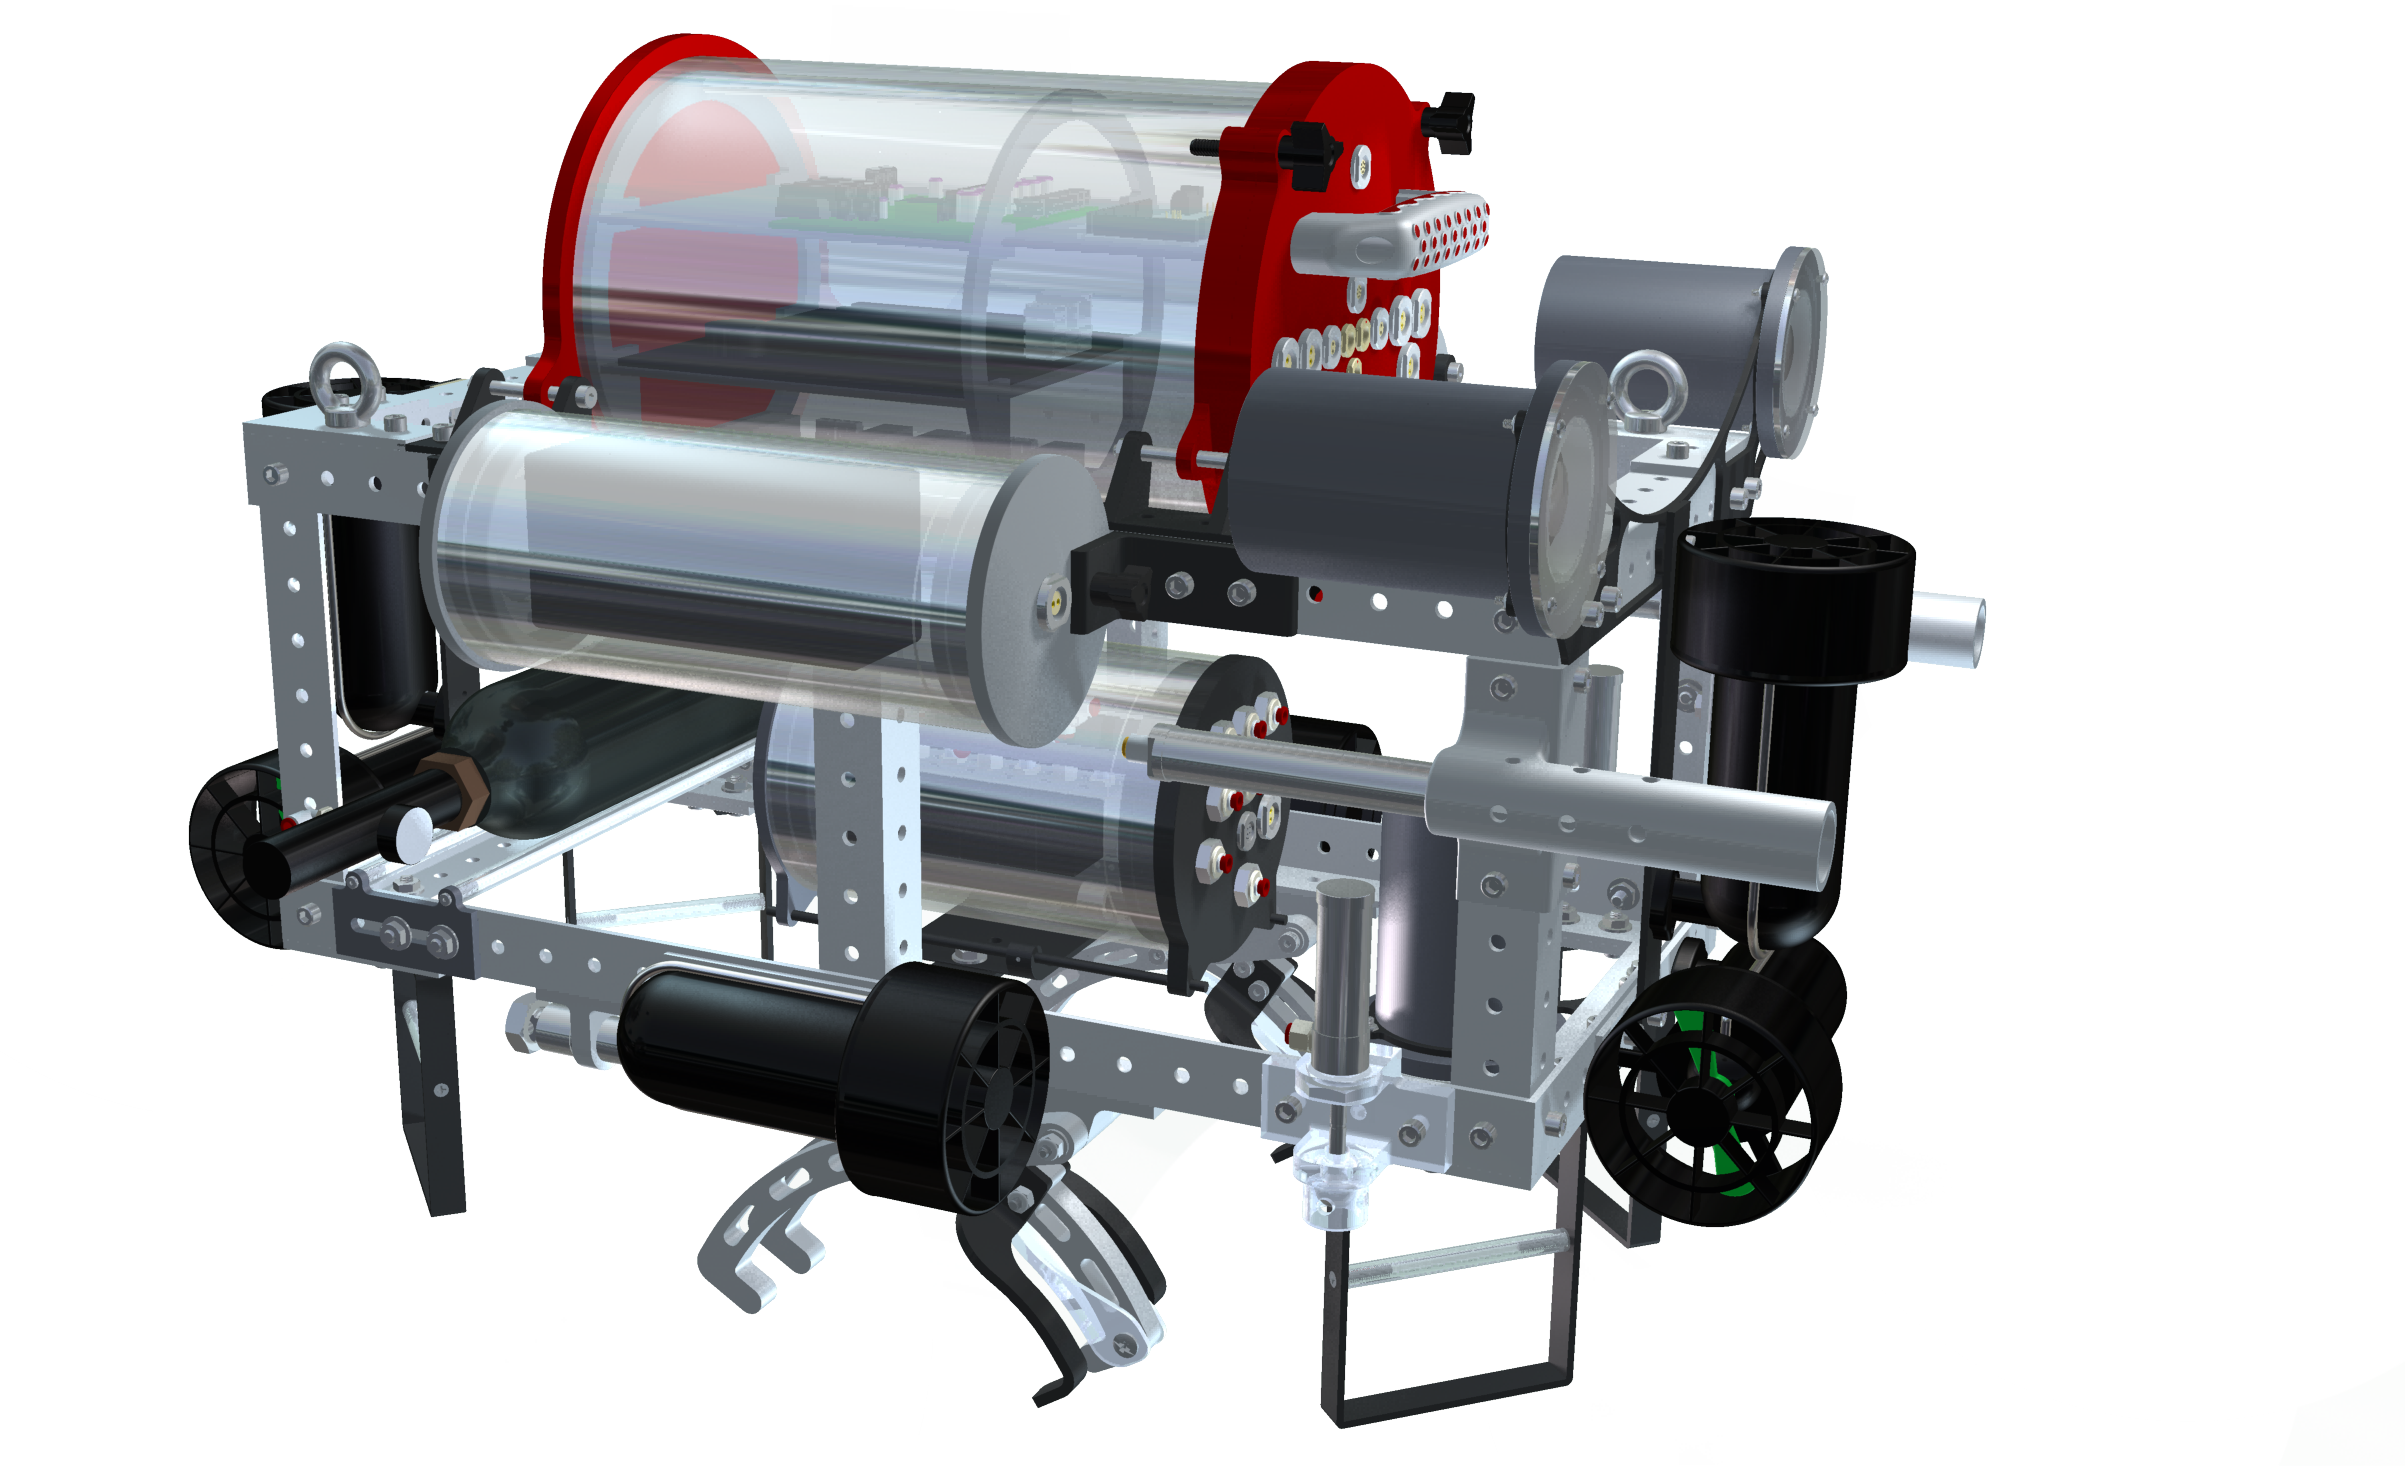
\includegraphics[height=4.2in]{media/full_assembly.png}
			\caption{AUV assembly}
			\label{auv_assembly}
		\end{figure}

		Figure~\ref{auv_assembly} shows the current CAD model of the entire AUV. It consists of a frame, a main hull pressure vessel, two battery pressure vessels, three camera pressure vessels, a pneumatic valve housing, an IMU pressure vessel, two claw mechanisms, two marker dropping devices, two pneumatic torpedoes, a $CO_2$ tank, and six thrusters.  The majority of the materials are HDPE plastic, 3D-printed resin, and aluminum.  All designs are from scratch, except for fasteners and electrical components. 
	\end{samepage}


	\begin{samepage}
		\begin{figure}[H]
			\centering
			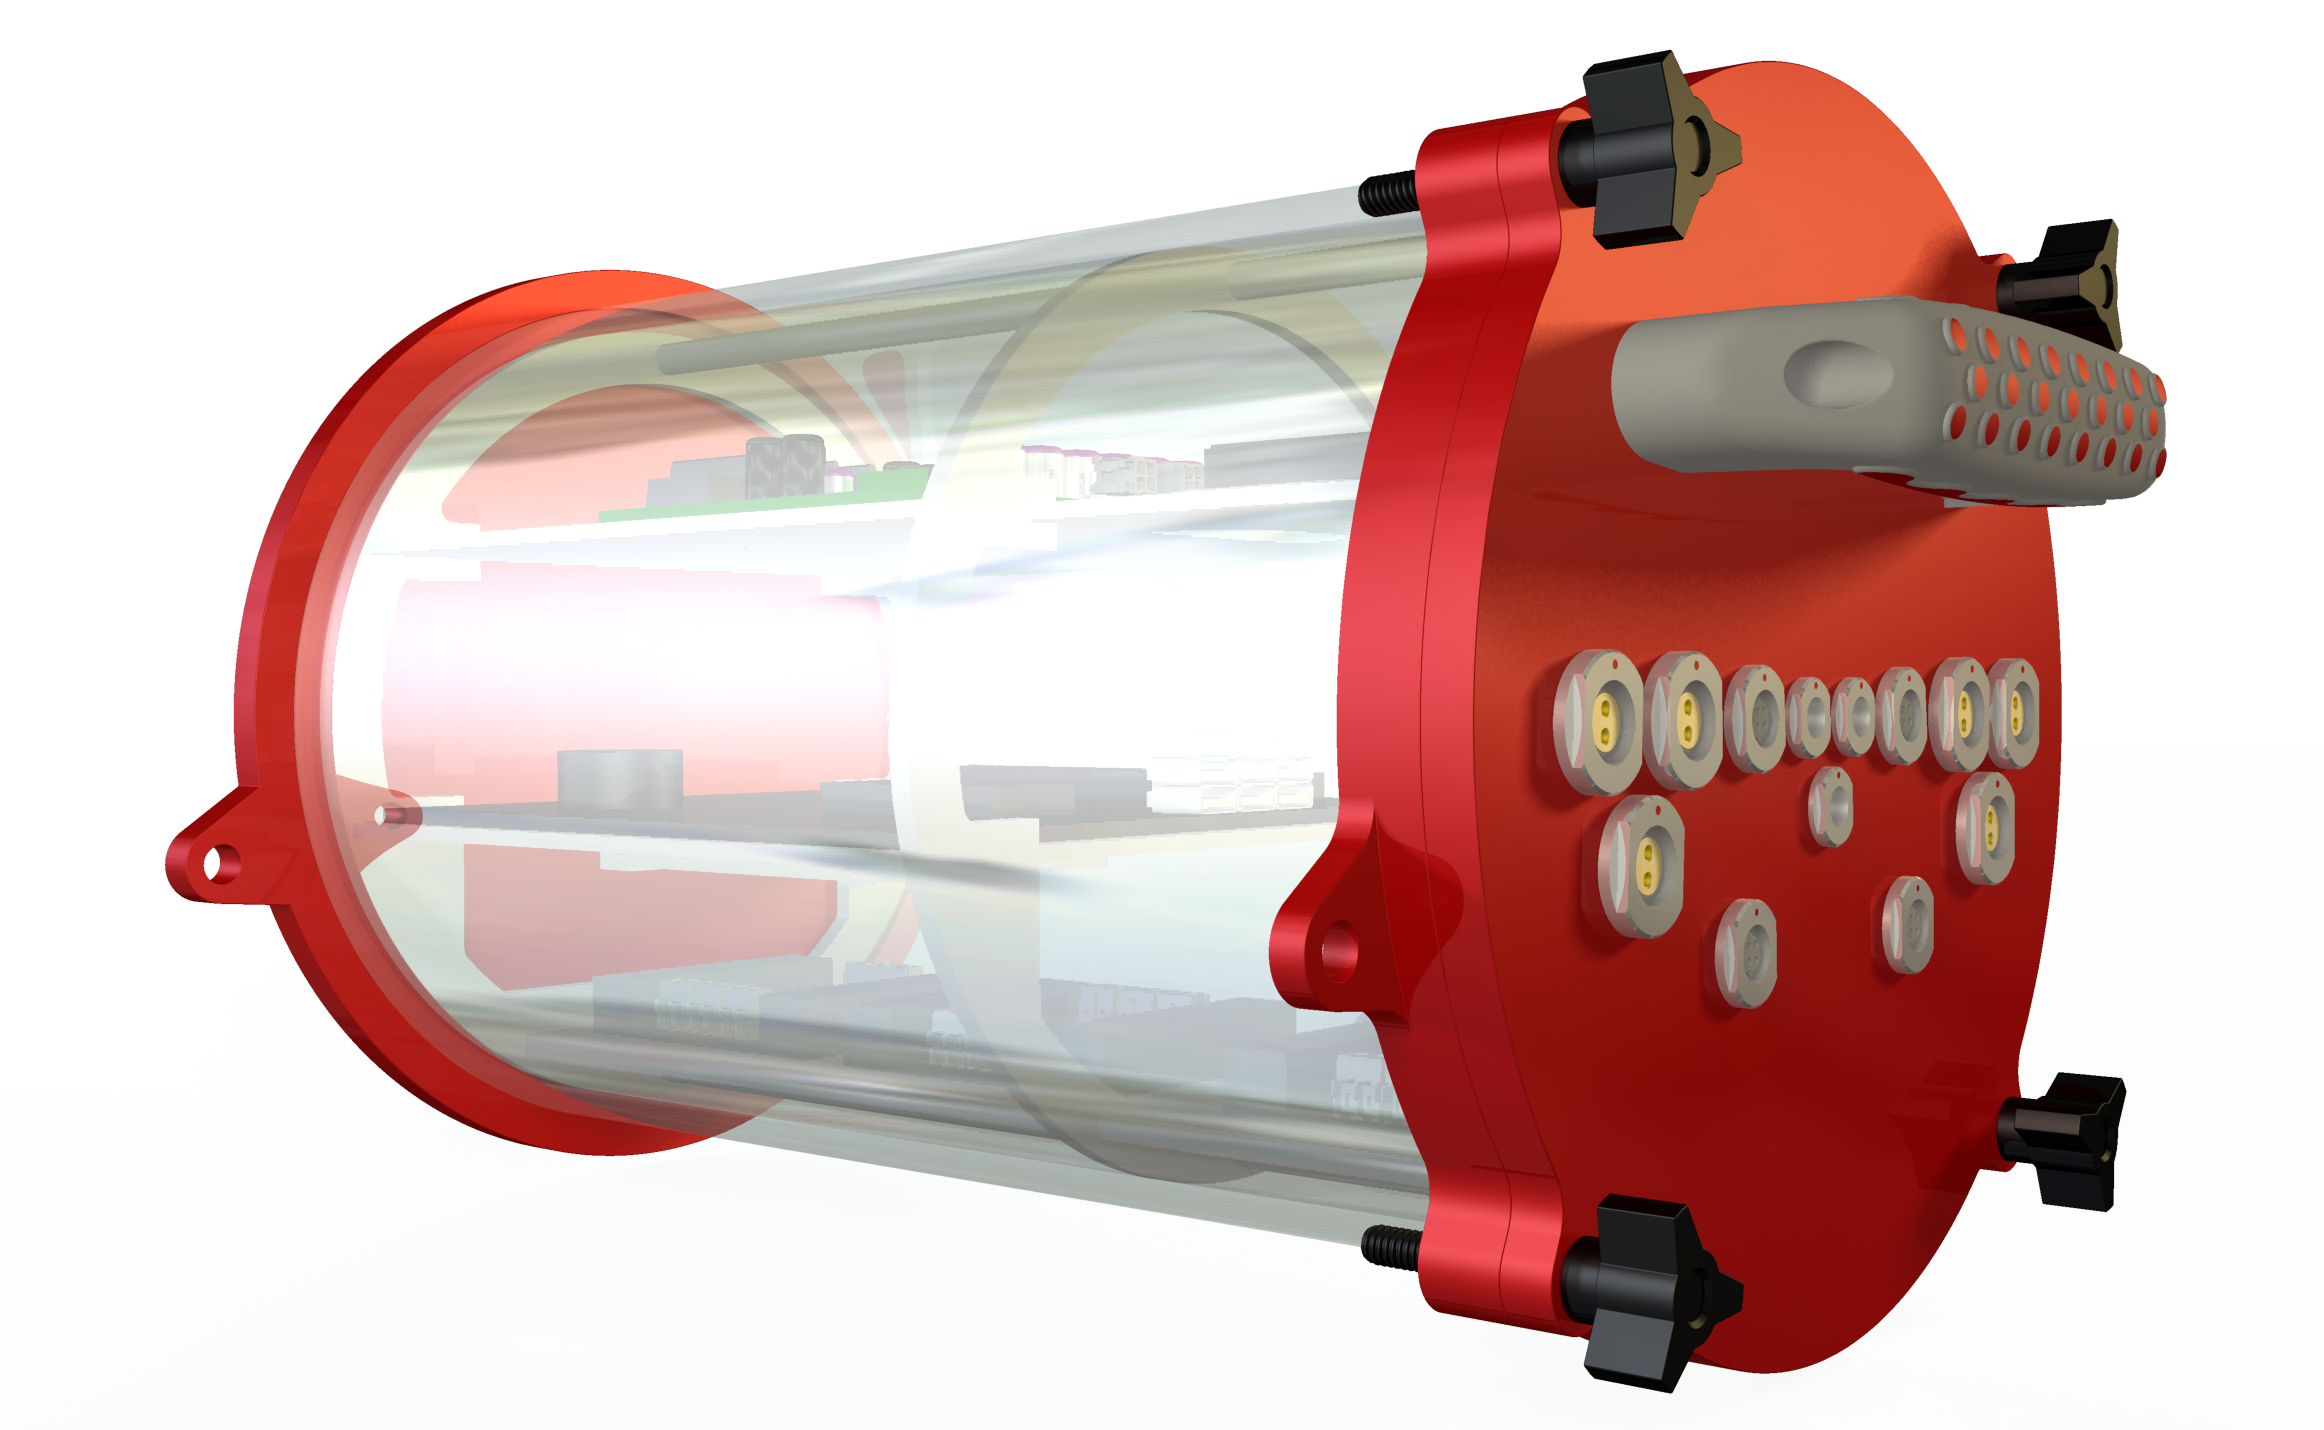
\includegraphics[height=4in]{media/main_hull.png}
			\caption{Main hull pressure vessel}
			\label{main_hull}
		\end{figure}

		The main hull houses most of the electronics and provides the majority of the buoyant force needed to keep the vehicle neutral and balanced. Inside, a rail system holds the electronics in place, and is removable from the front for easy access.  It attaches to the top of the frame, and connects all the electronic components using a set of waterproof connectors. 
	\end{samepage}

	\begin{figure}[H]
		\centering
		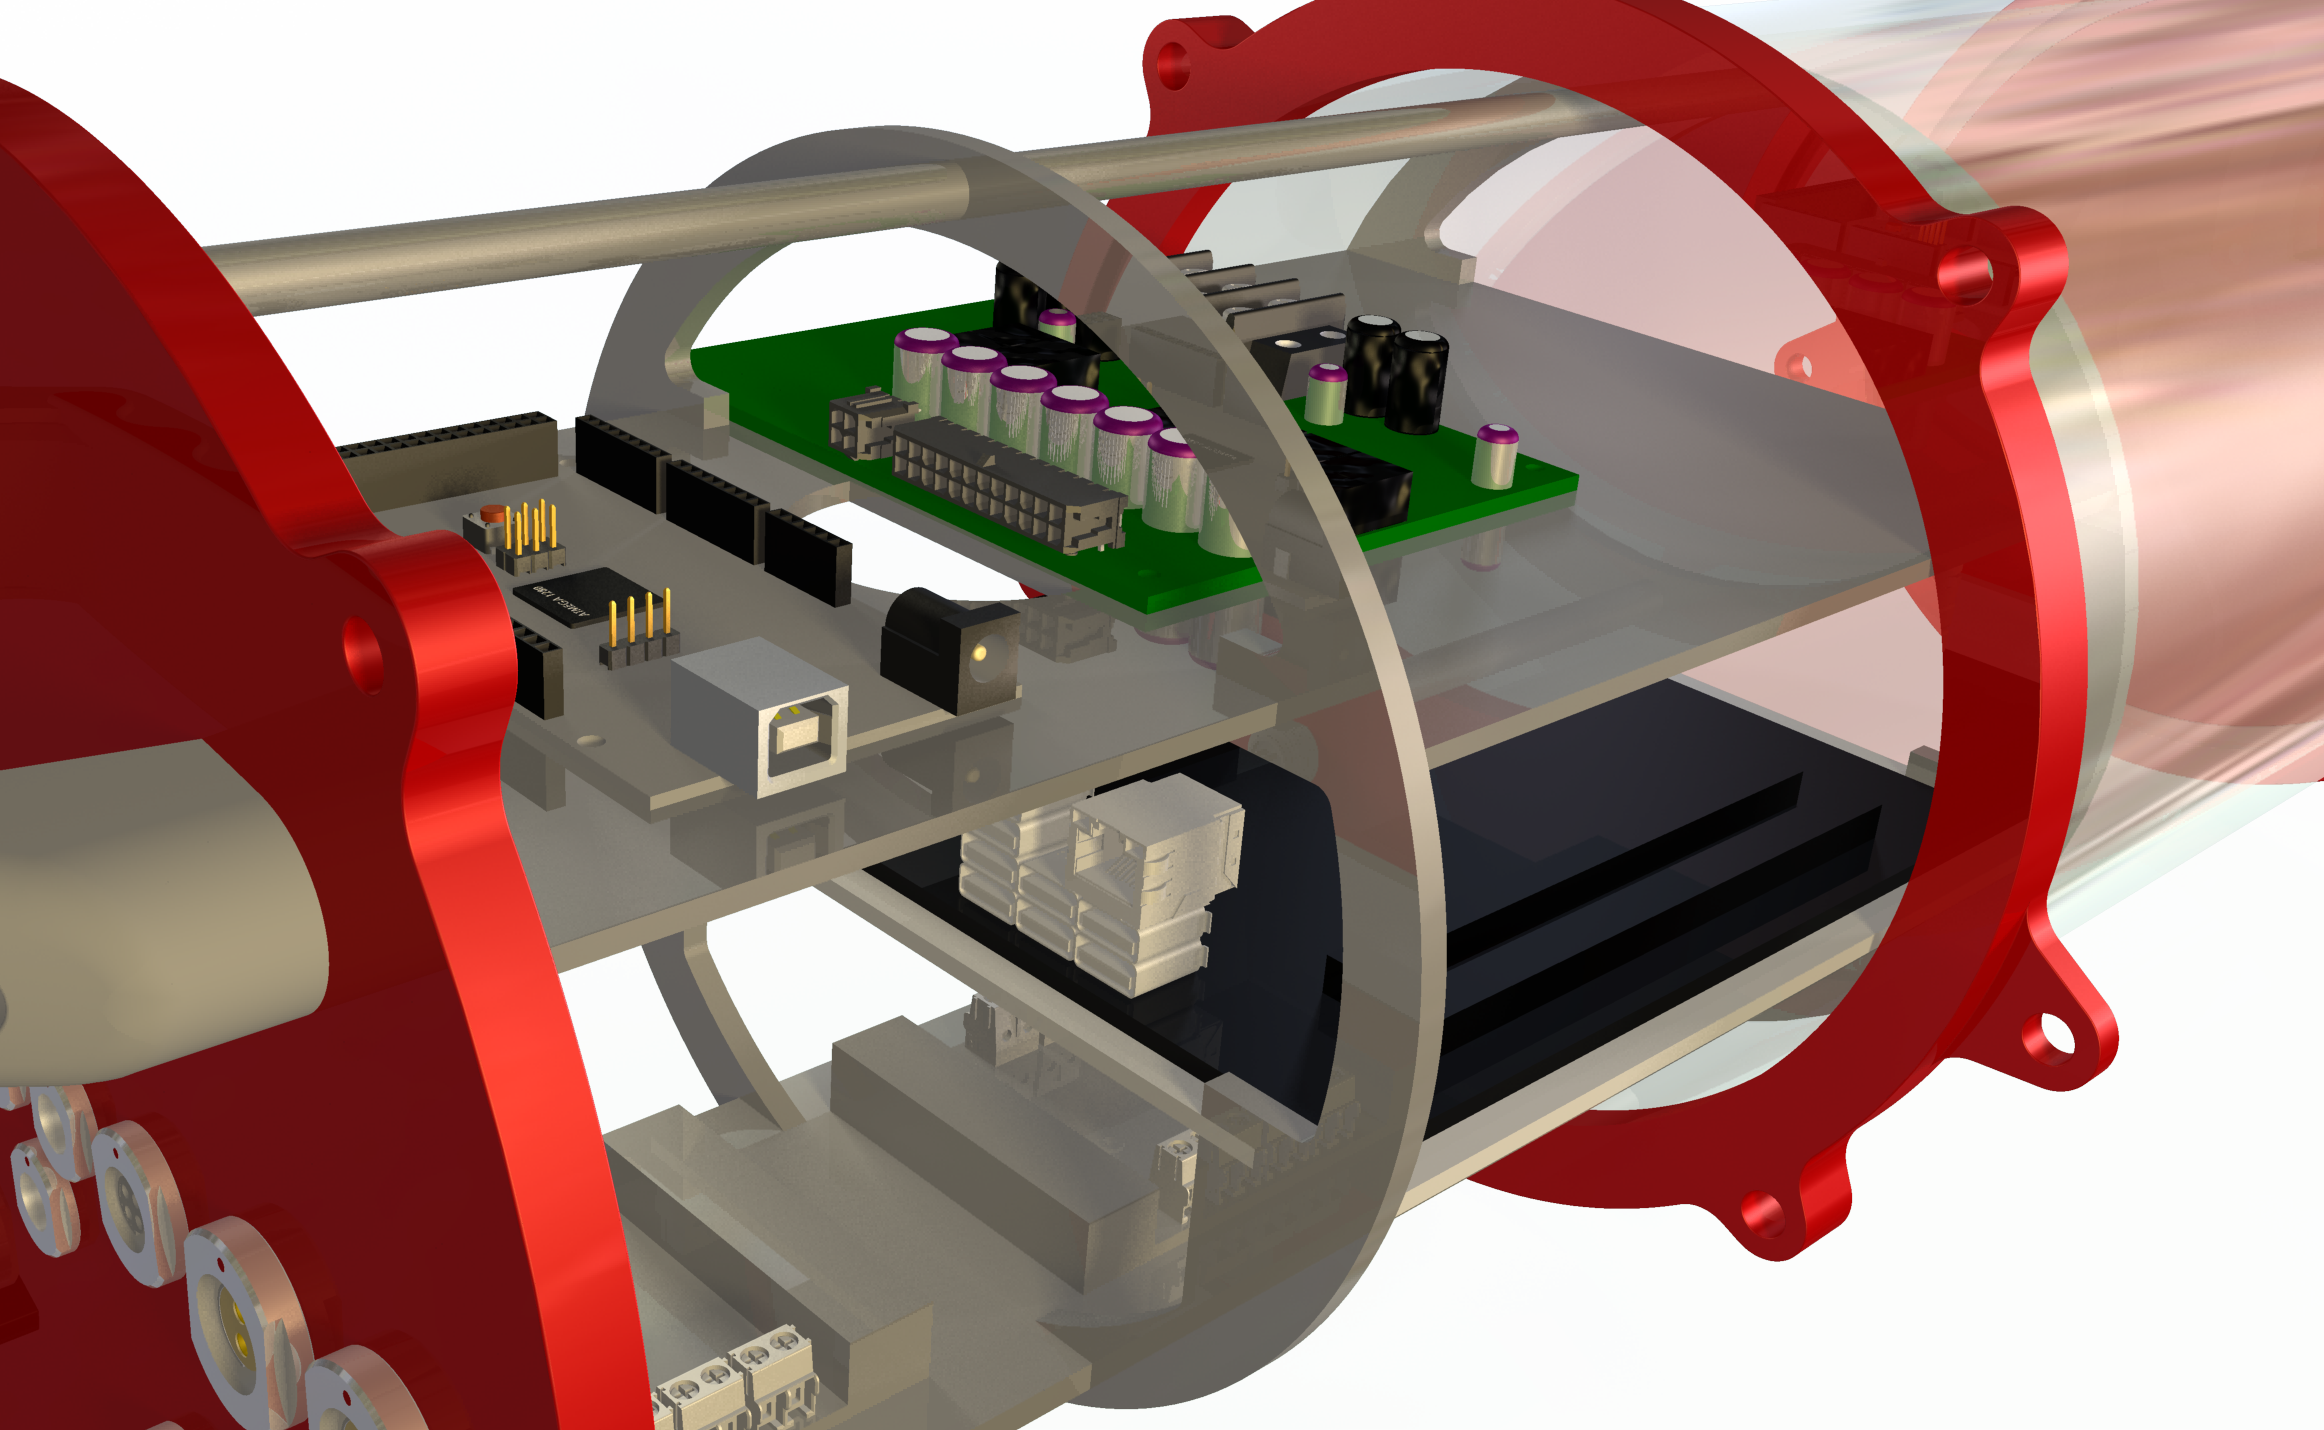
\includegraphics[height=4in]{media/MAIN-HULL-RENDER-2-ALPHA.png}
		\caption{Internal electronics rack}
		\label{main_hull2}
	\end{figure}

	Inside is the custom-built, on-board computer, as well as three motor controllers, an Arduino Mega, and a custom-built power distribution PCB board.  These electronics are needed to manage the six thrusters, the sensor array, and the computer vision system.  The frame is made of aluminum rails, with plastic racks, and uses a face O-ring with four nuts and vacuum seal to keep it water-tight. 

	\begin{figure}[H]
		\centering
		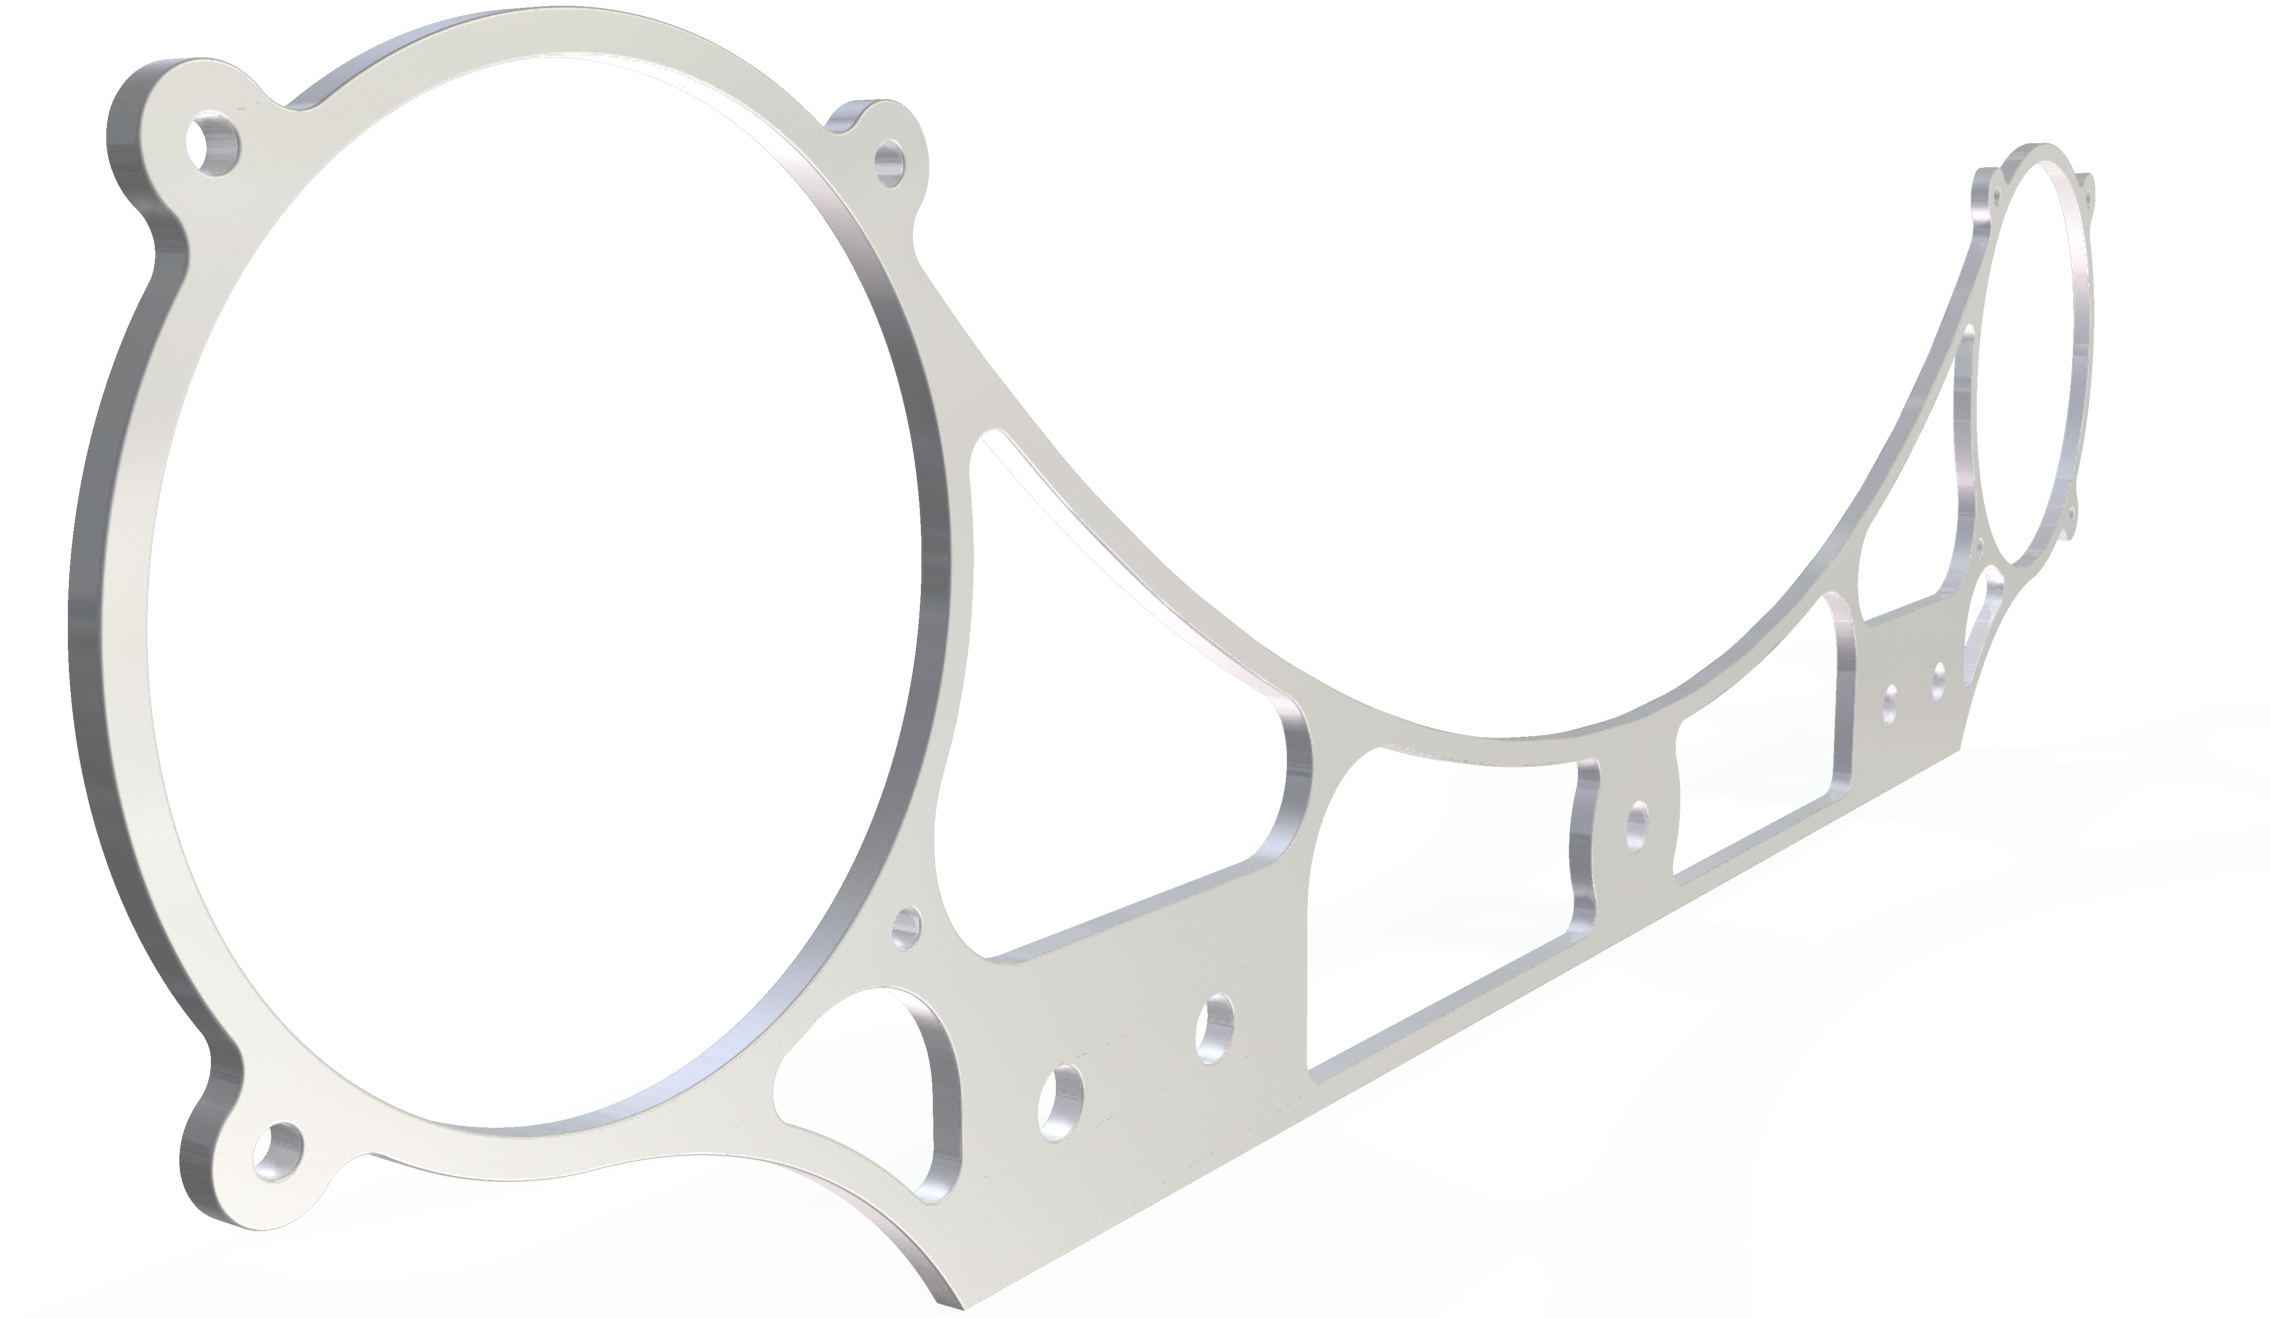
\includegraphics[height=4in]{media/front_camera_bracket.png}
		\caption{Front-facing CNCed camera bracket}
		\label{camera_bracket}
	\end{figure}

	The front-facing camera bracket connects two cameras to the bow to allow for stereo vision.  The bracket is CNCed from a sheet of aluminum for rigidity and shaped to maximize the distance between the cameras and reduce weight.  Like all the machined aluminum parts, it will be anodized following machining to prevent corrosion.


\end{document}